% Simulations
\chapter{Anomaly Response Simulations}  \label{ch:numerical}
\section{SISO State Feedback and On-Board Pilot}
% TODO make sure notation here is consistent with earlier

The shared control solution introduced in Chapter \ref{ch:siso_shared_ctrl} is applied to the problem introduced in Section \ref{sec:siso_problem}, using a simulation model of the lateral-directional dynamics of a fixed-wing aircraft and making assumptions about the perceptive capabilities and actions of an on-board human pilot. The aircraft model used in simulation is described in Section \ref{subsec:latdir_model}. The results of numerical simulations of the control of this plant and recovery from the two anomalies -- actuators whose dynamics change abruptly from a DC gain to first-order, and sensors whose measurements abruptly become time-delayed -- are presented in Sections \ref{subsec:siso_act_sims} and \ref{subsec:siso_delay_sims}, respectively.

% TODO add comparisons to passive response for both
\subsection{Aircraft Rolling Mode Dynamics} \label{subsec:latdir_model}
This section describes the lateral-directional dynamics of a fixed-wing aircraft. For an aircraft in steady wings-level flight with equilibrium speed $V_0$, pitch angle $\theta_0$, and no sideslip ($\beta_0 = 0$), and assuming small perturbations about the equilibrium point, the lateral-directional dynamics of the aircraft can be decoupled from the longitudinal aircraft dynamics, and linearized as follows \cite{stevens2015aircraft}:
%\begin{eqnarray}
%	x_{\mathrm{lat}} &=& \begin{bmatrix}\beta & \phi_s & p_s & r_s \end{bmatrix}^T, \qquad u_{\mathrm{lat}} = \begin{bmatrix}\delta_a & \delta_r \end{bmatrix}^T \nonumber \\
%	A_{\mathrm{lat}} &=& \begin{bmatrix}
%			\frac{Y_\beta}{V_0} & \frac{g_D\cos{\theta_0}}{V_0} & \frac{Y_p}{V_0} & \frac{Y_r}{V_0} - 1 \\
%			0 & 0 & \frac{1}{\cos{\theta_0}} & 0 \\
%			L_\beta & 0 & L_p & L_r \\
%			N_\beta & 0 & N_p & N_r
%		\end{bmatrix}, \qquad B_{\mathrm{lat}} = \begin{bmatrix}
%			\frac{Y_{\delta_a}}{V_0} & \frac{Y_{\delta_r}}{V_0} \\
%			0 & 0 \\
%			L_{\delta_a} & L_{\delta_r} \\
%			N_{\delta_a} & N_{\delta_r} 
%		\end{bmatrix}
%\end{eqnarray}
\begin{equation}
	\underbrace{\begin{bmatrix}\dot \beta \\ \dot \phi_s \\ \dot p_s \\ \dot r_s \end{bmatrix}}_{\dot{x}_{\mathrm{lat}}} = \underbrace{\begin{bmatrix}
			\frac{Y_\beta}{V_0} & \frac{g_D\cos{\theta_0}}{V_0} & \frac{Y_p}{V_0} & \frac{Y_r}{V_0} - 1 \\
			0 & 0 & \frac{1}{\cos{\theta_0}} & 0 \\
			L_\beta & 0 & L_p & L_r \\
			N_\beta & 0 & N_p & N_r
		\end{bmatrix}}_{A_{\mathrm{lat}}}
		\underbrace{\begin{bmatrix} \beta \\ \phi_s \\ p_s \\ r_s \end{bmatrix}}_{\dot{x}_{\mathrm{lat}}} + 
		\underbrace{\begin{bmatrix}
			\frac{Y_{\delta_a}}{V_0} & \frac{Y_{\delta_r}}{V_0} \\
			0 & 0 \\
			L_{\delta_a} & L_{\delta_r} \\
			N_{\delta_a} & N_{\delta_r} 
		\end{bmatrix}}_{B_{\mathrm{lat}}} 
		\underbrace{\begin{bmatrix}\delta_a \\ \delta_r \end{bmatrix}}_{u_{\mathrm{lat}}}
\end{equation}
\noindent where derivations of the stability and control derivatives in matrices $A_{\mathrm{lat}}$ and $B_{\mathrm{lat}}$ can be found in other references (see Refs.~\cite{stevens2015aircraft} or \cite{lavretsky2013robust} for more details). The states correspond to sideslip angle, stability axis bank angle, stability axis roll rate, and stability axis yaw rate, respectively, while the control inputs correspond to aileron and rudder deflections.

Based on time-scale separation, second-order dynamics of aileron-to-roll-angle are extracted from this fourth-order system and denoted here as the rolling mode dynamics, given by
\begin{equation}
	\underbrace{\begin{bmatrix}
			\dot{\phi} \\ \dot{p}
		\end{bmatrix}}_{\dot{x}_p} = \underbrace{\begin{bmatrix}
			0 & 1 \\ 0 & L_p
		\end{bmatrix}}_{A_p} \underbrace{\begin{bmatrix}
			\phi \\ p
		\end{bmatrix}}_{x_p} + \underbrace{\begin{bmatrix}
			0 \\ L_{\delta_a}
		\end{bmatrix}}_{B_p} \underbrace{\delta_a}_{u_p}.
	\label{eqn:2nd_order_lateral}
\end{equation}
This system corresponds to the plant as in (\ref{eq:siso_plant}), and it is noted that the rolling mode dynamics has the following transfer function in the Laplace frequency domain:
\begin{equation}
		\frac{\Phi(s)}{\Delta_a(s)} = \frac{L_{\delta_a}}{s^2 - L_p s}.
\end{equation}

In these equations, $\delta_a$ represents aileron input, and $\phi$ and $p$ denote the aircraft bank angle and roll rate in stability axes, with the subscript $(\cdot)_s$ dropped for notational simplicity. It is assumed that the states ($x_p$) are fully available for feedback (directly from sensors for $p$, and via integration of $p$ for $\phi$). $L_p$ is the roll damping derivative and $L_{\delta_a}$ is the rolling moment due to aileron deflection. We consider scenarios in which these parameters may be unknown, but are addressed in normal operation by an adaptive autopilot. The system has been simplified by fixing $\delta_r(t) = 0$ (no rudder input), so that aileron deflection is the only input. In normal operation, we assume the vehicle has sufficiently fast actuators, so that $\delta_a(t) = u(t)$ and equivalently $\Delta_a(s) = U(s)$, where $u(t)$ is the control signal. 

Under nominal vehicle operation with the plant given by (\ref{eqn:2nd_order_lateral}), a second-order reference model corresponding to (\ref{eqn:crm}) is used
\begin{equation}
	\underbrace{\begin{bmatrix}
		\dot{\phi}_d \\ \dot{p}_d
	\end{bmatrix}}_{\dot{x}_m} = \underbrace{\begin{bmatrix}
		0 & 1\\ -a_{m,1} & -a_{m,2}
	\end{bmatrix}}_{A_m} \underbrace{\begin{bmatrix}
		\phi_d \\ p_d
	\end{bmatrix}}_{x_m} + \underbrace{\begin{bmatrix}
		0 \\ b_{m,2}
	\end{bmatrix}}_{B_m} r(t) - L_m e(t)
	\label{eqn:rm_2_symbolic}
\end{equation}
\noindent where $x_m(t)$ is a vector of the desired states, $e(t) = x_p(t) - x_m(t)$ is the model-following error, and $r(t)$ is the commanded bank angle. It is straightforward to see that a choice of
\begin{eqnarray}
	\theta^* &=& \Big[ \frac{-a_{m,1}}{L_{\delta_a}} \quad \frac{-a_{m,2}-L_p}{L_{\delta_a}} \Big] \label{e:tstar}\\
	q^* &=& \frac{b_{m,2}}{L_{\delta_a}} \label{e:qstar}
\end{eqnarray} 
\noindent solves the matching condition in (\ref{eqn:matchcond1}) and (\ref{eqn:matchcond2}). This in turn implies that even if the roll damping derivative ($L_p$) and the rolling moment due to aileron deflection ($L_{\delta_a}$) are unknown, the adaptive controller in (\ref{eqn:control_law}), (\ref{eqn:thetadot_projection}), and (\ref{eqn:qdot_projection}) will be able to vary the feedback and feedforward gains such that the closed-loop response of the system is satisfactory. We shall denote such a case as nominal operation, and consider the anomalous cases as those where in addition to parametric uncertainties, changes in dynamics as described in Sections \ref{subsec:siso_act_fault} and \ref{subsec:siso_delay} occur.

% TODO make sure notation here is consistent with earlier
Numerical data for the Boeing 747 flying straight-and-level at Mach 0.25 at sea level \cite{heffley1972aircraft} was substituted into (\ref{eqn:2nd_order_lateral}) to constitute the following nominal plant dynamics,
\begin{equation}
		\underbrace{\begin{bmatrix}
			\dot{\phi} \\ \dot{p}
		\end{bmatrix}}_{\dot{x}_p} = \underbrace{\begin{bmatrix}
			0 & \hfil 1 \\ 0 & -1.10
		\end{bmatrix}}_{A_p} \underbrace{\begin{bmatrix}
			\phi \\ p
		\end{bmatrix}}_{x_p} + \underbrace{\begin{bmatrix}
			0 \\ 0.318
		\end{bmatrix}}_{B_p} \delta_a \label{eqn:siso_plant_nominal_num}
\end{equation} \noindent which results in the open-loop transfer function 
\begin{equation}
		\frac{\Phi(s)}{\Delta_a(s)} = \frac{0.318}{s^2 + 1.10s}. 
\end{equation}
A closed-loop reference model, corresponding to (\ref{eqn:rm_2_symbolic}), is designed with the following numerical values
\begin{equation}
	\dot{x}_m = \underbrace{\begin{bmatrix}
		\hfil 0 & \hfil 1\\ -8 & -6
	\end{bmatrix}}_{A_m} x_m + \underbrace{\begin{bmatrix}
		0 \\ 8
	\end{bmatrix}}_{B_m} r - \underbrace{\begin{bmatrix}
		\hfil -10 & \hfil -1 \\ \hfil 8 & \hfil -4
	\end{bmatrix}}_{L_m} e
	\label{eqn:rm_2}
\end{equation}
\noindent for use with the nominal adaptive controller. The initial feedback and feedforward parameters used in simulation, $\theta(t=0)$ and $q(t=0)$, are chosen such that the matching conditions of (\ref{e:tstar}) and (\ref{e:qstar}) are met.

The two cases of anomalies discussed in Sections \ref{subsec:siso_act_fault} and \ref{subsec:siso_delay}, of the introduction of actuator dynamics and a time delay, respectively, were simulated numerically in MATLAB/Simulink for bank angle tracking tasks. In these simulations, the commanded stability axis bank angle is a sequence of 5-second steps. In the simulations of these two types of anomalies, which are presented in Sections \ref{subsec:siso_act_sims} and \ref{subsec:siso_delay_sims}, the anomaly is assumed to occur at $t_1^* = 30$s, and the corrective action is applied to the controller at $t_2^* = 90$s. Time $t_3^*$ denotes the time when failure of the aircraft is assumed to occur, if applicable. The three anomaly response (AR) simulations to be presented are summarized as follows.
\begin{description}
	\item[Act-AR (Shared)] Simulation of a shared control response to an anomaly which causes a plant with parametric uncertainties to abruptly undergo a change in actuator dynamics from direct gain to first-order lag
	\item[Del-AR (Shared)] Simulation of a shared control response to an anomaly which introduces a time delay into the measurement of the state of a plant with parametric uncertainties
	\item[Del-AR-P (Passive)] Simulation of a passive response to an anomaly which introduces a time delay into the measurement of the state of a plant with parametric uncertainties, and the nominal adaptive autopilot retains control without intervention from the remote human supervisor
\end{description}

\subsection{Actuator Fault}\label{subsec:siso_act_sims}
The first anomaly considered in simulation (\textbf{Act-AR}), corresponding to the problem stated in Section \ref{subsec:siso_act_fault}, is the abrupt occurrence of an actuator fault, which is assumed to change the actuator dynamics from a direct gain (\ref{eq:siso_plant_input_nom}) to a first-order lag (\ref{eqn:actuator_dynamics_symbolic}). By applying the change in dynamics defined in (\ref{eqn:actuator_dynamics_symbolic}), and choosing $T_l = 1.0$s, the plant dynamics change from (\ref{eqn:siso_plant_nominal_num}) to
\begin{equation}
	\underbrace{\begin{bmatrix}
			\dot{\phi} \\ \dot{p} \\ \ddot{p}
		\end{bmatrix}}_{\dot{x}_p'} = \underbrace{\begin{bmatrix}
		0 & \hfil 1 & \hfil 0\\ 0 & \hfil 0 & \hfil 1 \\ 0 & -1.10 & -2.10
	\end{bmatrix}}_{A_p'} \underbrace{\begin{bmatrix}
			\phi \\ p \\ \dot{p}
		\end{bmatrix}}_{x_p'} + \underbrace{\begin{bmatrix}
		0 \\ 0 \\ 0.318
	\end{bmatrix}}_{B_p'} u
	\label{eqn:plant_3}
\end{equation}
\noindent at $t = t_1^*$, corresponding to the higher-order plant model given by (\ref{eqn:plant_3_compact}). This results in the open-loop transfer function
\begin{equation}
		\frac{\Phi(s)}{U(s)} = \frac{0.318}{s^3 + 2.10s^2 + 1.10s}.\\
\end{equation}

Using this pilot input, we propose an adaptive controller predicated on a third-order dynamics of the open-loop plant and assume that in addition to the bank angle and roll rate, angular acceleration $\dot{p}$ is also measurable. We choose a reference model as
\begin{equation}
	\underbrace{\begin{bmatrix}
		\dot{\phi}_d \\ \dot{p}_d \\ \ddot{p}_d
	\end{bmatrix}}_{\dot{x}_m'} = \underbrace{\begin{bmatrix}
		\hfil 0 & \hfil 1 & \hfil 0\\ \hfil 0 & \hfil 0 & \hfil 1 \\ -32 & -32 & -10
	\end{bmatrix}}_{A_m'} \underbrace{\begin{bmatrix}
		\phi_d \\ p_d \\ \dot{p}_d
	\end{bmatrix}}_{x_m'} + \underbrace{\begin{bmatrix}
		0 \\ 0 \\ 32
	\end{bmatrix}}_{B_m'} r - \underbrace{\begin{bmatrix}
		-10 & -1 & \hfil 0 \\ \hfil 0 & -10 & -1 \\ \hfil 32 & \hfil 32 & \hfil 0
	\end{bmatrix}}_{L_m'} e'
	\label{eqn:rm_3}
\end{equation}

After detection and diagnosis of the anomaly with the shared decision-making framework, the corrective action to increase the dimension of the controller is made at $t = t_2^*$, and the reference model dynamics is switched to that of (\ref{eqn:rm_3}).
%\begin{equation}
%	\dot{x}_m' =  \underbrace{\begin{bmatrix}
%		\hfil 0 & \hfil 1 & \hfil 0\\ \hfil 0 & \hfil 0 & \hfil 1 \\ -32 & -32 & -10
%	\end{bmatrix}}_{A_m'} x_m' + \underbrace{\begin{bmatrix}
%		0 \\ 0 \\ 32
%	\end{bmatrix}}_{B_m'} r - \underbrace{\begin{bmatrix}
%		-10 & -1 & \hfil 0 \\ \hfil 0 & -10 & -1 \\ \hfil 32 & \hfil 32 & \hfil 0
%	\end{bmatrix}}_{L_m'} e'
%	\label{eqn:rm_3}
%\end{equation}
%
The control gains which will cause the closed-loop roll response to match the desired response exactly are
\begin{align}
	\theta^*(t) = & \begin{cases}
		\Big[ -25.16, \quad -15.41 \Big] & t < t_1^* \\
		\Big[-32.00, \quad -30.90, \quad -2.10 \Big] & t \geq t_1^*
	\end{cases} \\
	q^*(t) = & \begin{cases}
		25.16 & t < t_1^* \\
		32.00 & t \geq t_1^*
	\end{cases}
\end{align}
\noindent which are unknown to the adaptive controller. As mentioned earlier, initial values are chosen as $\theta(t=0)= [-25.16, \quad -15.41]$ and $q(t=0)=25.16$. The learning rates in (\ref{eqn:thetadot_projection}) and (\ref{eqn:qdot_projection}) were chosen to be $\Gamma_\theta = 10 I_2$, with $I_n$ the identity matrix of dimension $n$, and $\gamma_q = 10$. The projection operator was not used in this simulation. It was assumed that $t_1^*=30$s and $t_2^*=90$s. To add more realism to the simulation example, we have assumed that the signal $\dot{p}$ is not directly measured, and instead use a high-pass filter to estimate it from $p$ using $\hat{\dot{p}} = \frac{as}{s+a} p$. Results of this simulation are given in Figures \ref{fig:command_and_output}, \ref{fig:theta}, \ref{fig:error}, and \ref{fig:step_pole}. 

\begin{figure}[h!]
	\centering
	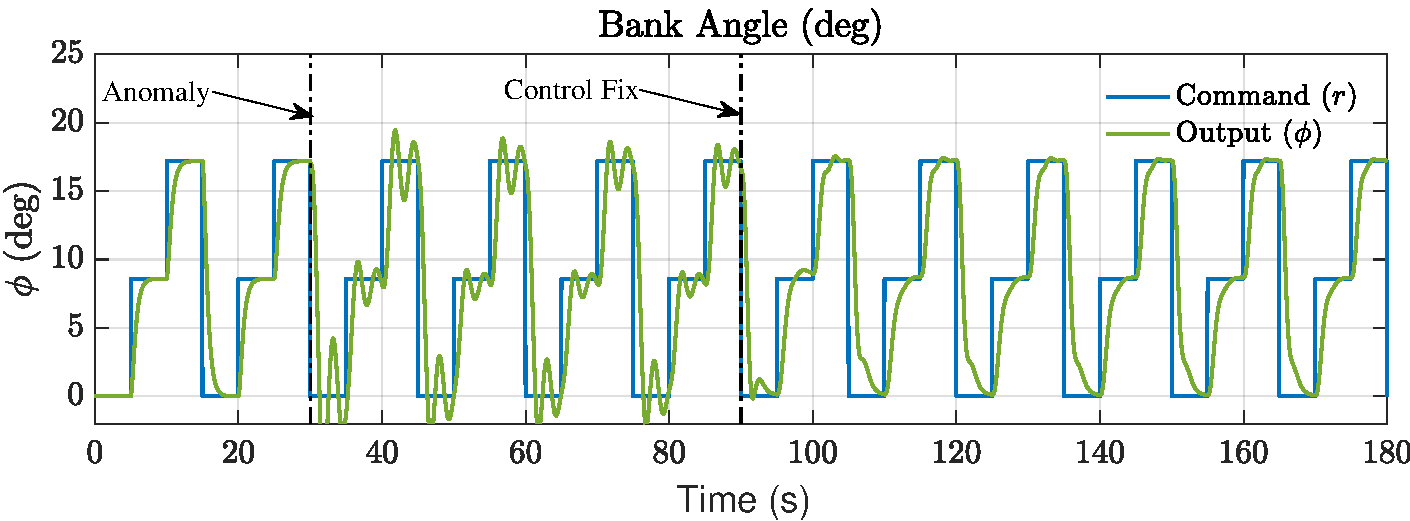
\includegraphics[width=\columnwidth]{phi_pole_v3.pdf}
	\caption{Act-AR simulation: Bank angle command ($r$) and output ($\phi$) under nominal operation ($t \leq t_1^*$), after change in actuator dynamics ($t_1^* < t \leq t_2^*$), and after a corrective action ($t > t_2^*$)}
	\label{fig:command_and_output}
\end{figure}

\begin{figure}[h!]
	\centering
	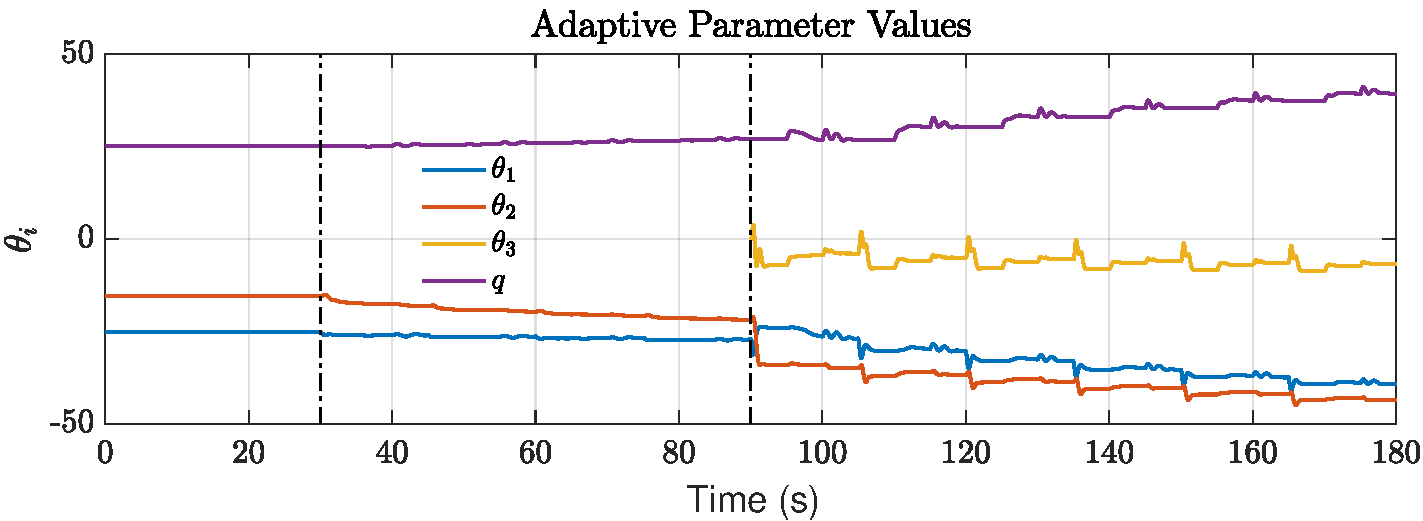
\includegraphics[width=\columnwidth]{theta_pole_v3.pdf}
	\caption{Act-AR simulation: Adaptive feedback gains under nominal operation ($t \leq t_1^*$), after change in actuator dynamics ($t_1^* < t \leq t_2^*$), and after a corrective action ($t > t_2^*$)}
	\label{fig:theta}
\end{figure}

\begin{figure}[h!]
	\centering
	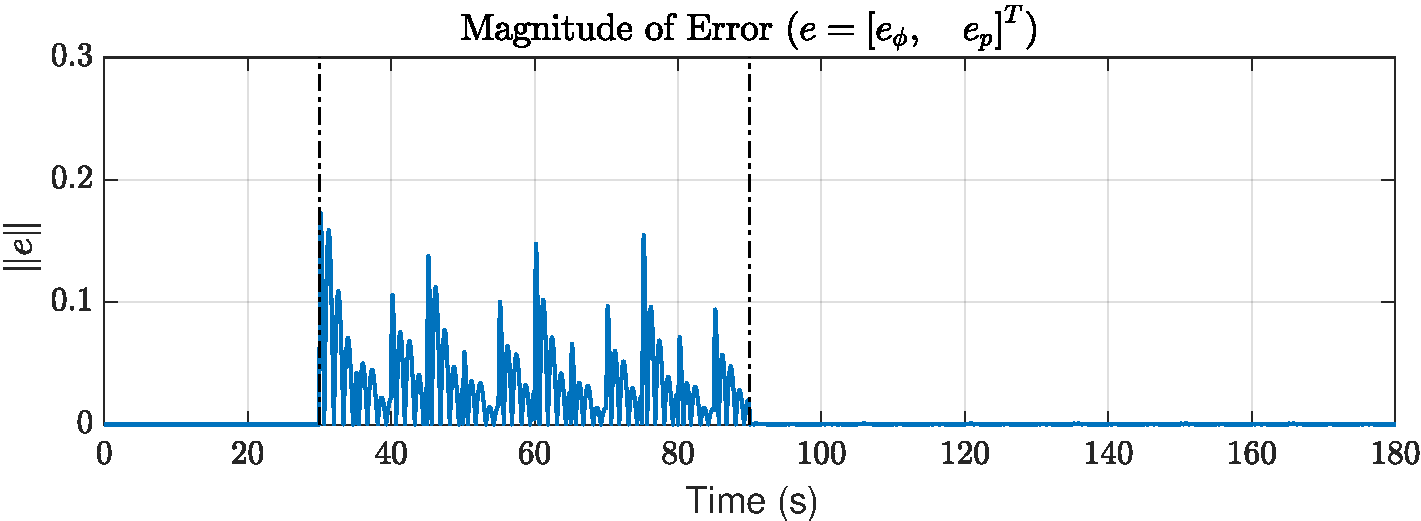
\includegraphics[width=\columnwidth]{e_pole_v3.pdf}
	\caption{Act-AR simulation: Tracking error $\|e\|$ under nominal operation ($t \leq t_1^*$), after change in actuator dynamics ($t_1^* < t \leq t_2^*$), and after a corrective action ($t > t_2^*$)}
	\label{fig:error}
\end{figure}

From Figures \ref{fig:command_and_output}, \ref{fig:theta}, and \ref{fig:error}, it is clear that after an initial adaptation period, the adaptive controller with third-order reference model dynamics converges on the desired feedback/feedforward gains, returning the roll control to its satisfactory performance without requiring any manual control from the human pilot. The action required from the human pilot is in the detection and diagnosis of the anomaly in dynamical behavior, leading to the addition of feedback on $\hat{\dot{p}}$ as a corrective action. 

% TODO better notation for "freezing" parameters
Taking average parameter values over time $\Delta t$ at the end of each stage of simulation (Nominal, Post-Anomaly, Post-Correction)
\begin{align}
	\bar{\theta}_{t_i} &= \frac{1}{\Delta t} \int_{t_{f,i}-\Delta t}^{t_{f,i}} \theta(t) dt, \qquad i = [1, 2, 3] \label{eqn:theta_bar}\\
	\bar{q}_{t_i} &= \frac{1}{\Delta t} \int_{t_{f,i}-\Delta t}^{t_{f,i}} q(t) dt, \qquad i = [1, 2, 3] \label{eqn:q_bar}
\end{align}
with $\Delta t = 5$s, $t_f = [30, \quad 90, \quad 180]$ allows us to define a closed-loop frequency response which is representative of controller performance after parameter adaptation in each stage. Figure \ref{fig:step_pole} shows the closed-loop unit step input responses with $(\bar{\theta}_i, \bar{q}_i)$ for $i = [1, 2, 3]$ plotted alongside the ideal response during nominal operation, demonstrating how the characteristics of nominal operation are recovered with the adaptive controller with three feedback parameters.

\begin{figure}[h!]
	\centering
	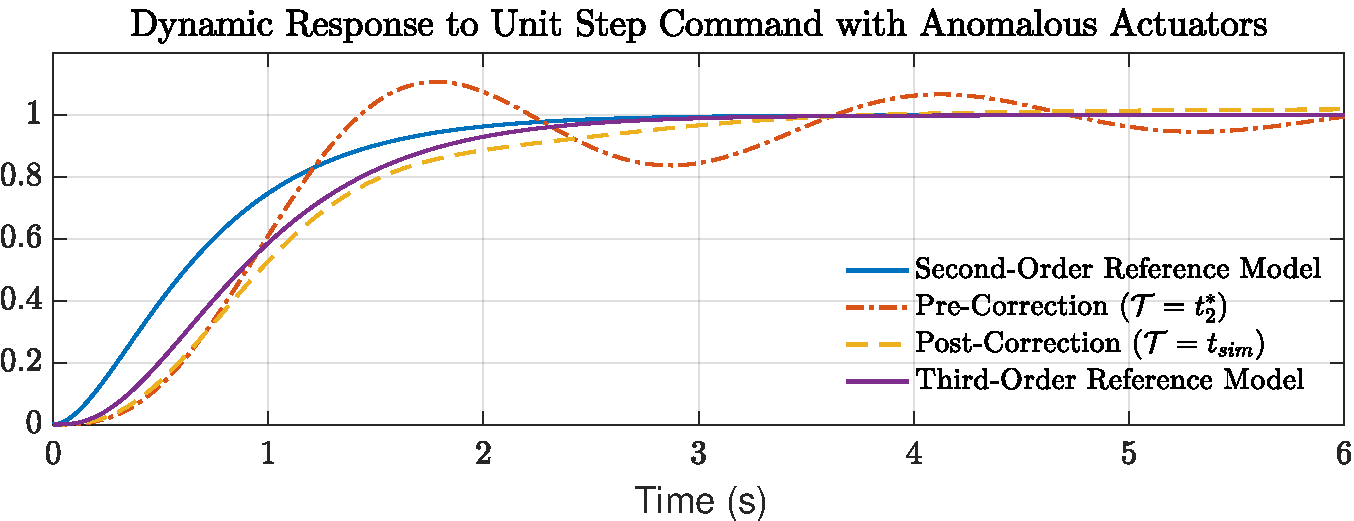
\includegraphics[width=\columnwidth]{step_pole_v3.pdf}
	\caption{Act-AR analysis: Unit step responses for closed-loop transfer functions at different stages of simulation, demonstrating performance improvement after corrective action}
	\label{fig:step_pole}
\end{figure}

\subsection{Time-Delayed Sensor Measurements}\label{subsec:siso_delay_sims}
The second type of anomaly considered in simulations (\textbf{Del-AR} and \textbf{Del-AR-P}), corresponding to the problem stated in Section \ref{subsec:siso_delay}, is the abrupt introduction of a time delay to sensor measurements. A time delay of $\tau = 0.200$s is added to the plant (\ref{eqn:2nd_order_lateral}) between the state measurements and their use in control input computation as in (\ref{eqn:delay_diffeq}), so that
\begin{equation}
	x_\sigma(t) = x_p(t - 0.20).
\end{equation}
With $\Phi_\sigma(s)$ defined as the delayed bank angle measurement, the change in the transfer function $\Phi_\sigma(s)/U(s)$ is thus
\begin{equation}
		\frac{\Phi_\sigma(s)}{U(s)} = \begin{cases}
			\frac{0.318}{s^2 + 1.10s} & t < t_1^*\\
			\frac{0.318}{s^2 + 1.10s}e^{-0.20 s} & t \geq t_1^*
		\end{cases} 
\end{equation}

For $0 < t < t_2^*$, the reference model used by the nominal adaptive controller in simulation is that given by (\ref{eqn:rm_2}). For $t \geq t_2^*$, the reference model used by the recovery adaptive controller in simulation is given by
\begin{equation}
	\underbrace{\begin{bmatrix}
		\dot{\phi}_d \\ \dot{p}_d \\ \ddot{p}_d
	\end{bmatrix}}_{\dot{x}_m'} = \underbrace{\begin{bmatrix}
		\hfil 0 & \hfil 1 & \hfil 0\\ \hfil 0 & \hfil 0 & \hfil 1 \\ -32 & -32 & -10
	\end{bmatrix}}_{A_m'} \underbrace{\begin{bmatrix}
		\phi_d \\ p_d \\ \dot{p}_d
	\end{bmatrix}}_{x_m'} + \underbrace{\begin{bmatrix}
		0 \\ 0 \\ 32
	\end{bmatrix}}_{B_m'} r - \underbrace{\begin{bmatrix}
		-10 & -1 & \hfil 0 \\ \hfil 0 & \hfil -10 & \hfil -1 \\ \hfil 32 & \hfil 32 & \hfil 9.9
	\end{bmatrix}}_{L_m'} e'.
	\label{eqn:rm_3_delay}
\end{equation}
Using the first-order delay approximation (\ref{eqn:delay_approx_diffeq}), given by
\begin{equation}
	0.20 \dot{x}_{\sigma}(t) + x_{\sigma}(t) = x_p(t),
\end{equation}
the feedback and feedforward gains which would give the desired closed-loop response for $\Phi_\sigma(s)/U(s)$ are
\begin{align}
	\theta^*(t) = & \begin{cases} \Big[-25.16, \quad -15.41 \Big] & t < t_1^* \\ 
	\Big[-20.13, \quad -16.67, \quad -2.45 \Big] & t \geq t_1^* \end{cases} \\
	q^*(t) = &\begin{cases} 25.16 & t < t_1^* \\ 20.13 & t \geq t_1^* \end{cases}
\end{align}

\noindent Parameter adaptation rates used in this simulation are given by
\begin{align}
	\Gamma_\theta  = & \begin{cases}
		10 I_2 & t < t_2^*\\
		\text{diag}(10.0, 10.0, 0.1) & t \geq t_2^*
 	\end{cases} \\
	\gamma_q  = &\quad 10.0 \qquad ~ \qquad ~ \qquad ~ \quad \forall t
\end{align}

\noindent where the learning rate on $\hat{\dot{p}}$ is lower than that used in the simulation of an actuator fault, to improve robustness to the first-order approximation used to model the time delay. In addition, a projection operator with the following constant parameters (\ref{eqn:proj_function}) was used to limit $\dot{\theta}(t)$
\begin{align}
	\varphi_m = & \begin{bmatrix}
		300, & 200, & 25
	\end{bmatrix} \\
	\varphi_{\epsilon} = & \begin{bmatrix}
		50, & 50, & 25
	\end{bmatrix}\end{align}
\noindent and the following constant parameters for the projection operator limiting $\dot{q}(t)$
\begin{align}
	\varphi_m = &~ 300\\
	\varphi_{\epsilon} = &~ 50
\end{align}

\begin{figure}[h!]
	\centering
	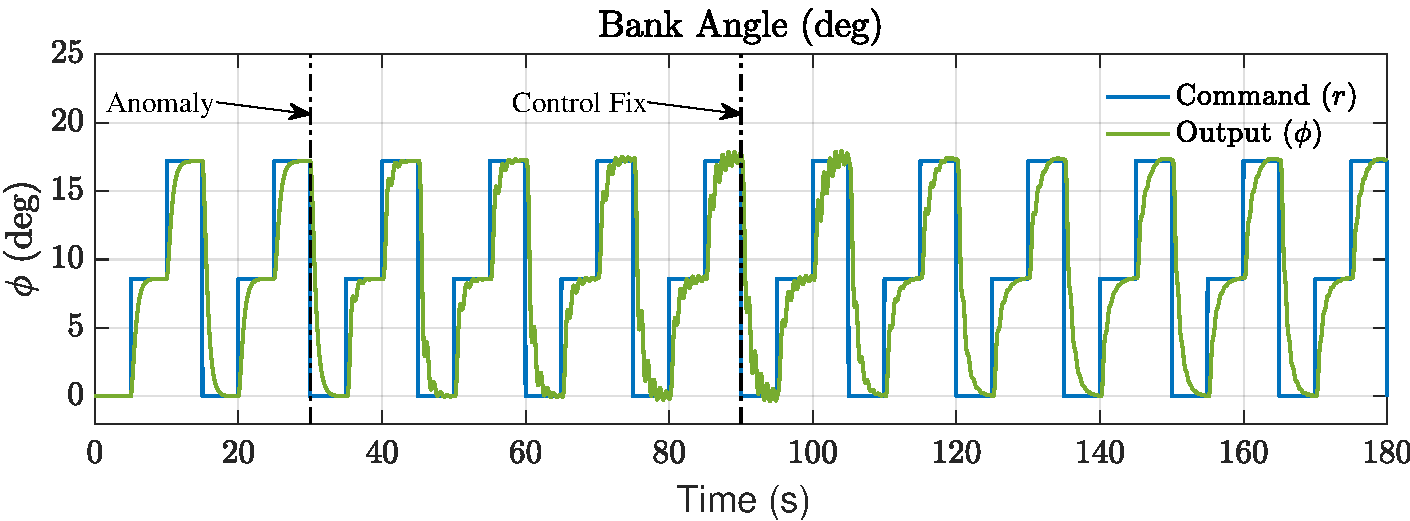
\includegraphics[width=\columnwidth]{phi_delay_v2.pdf}
	\caption{Del-AR simulation: Bank angle command ($r$) and output ($\phi$) under nominal operation ($t \leq t_1^*$), after abrupt addition of a time delay ($t_1^* < t \leq t_2^*$), and after a corrective action ($t > t_2^*$)}
	\label{fig:command_and_output_d}
\end{figure}

\begin{figure}[h!]
	\centering
	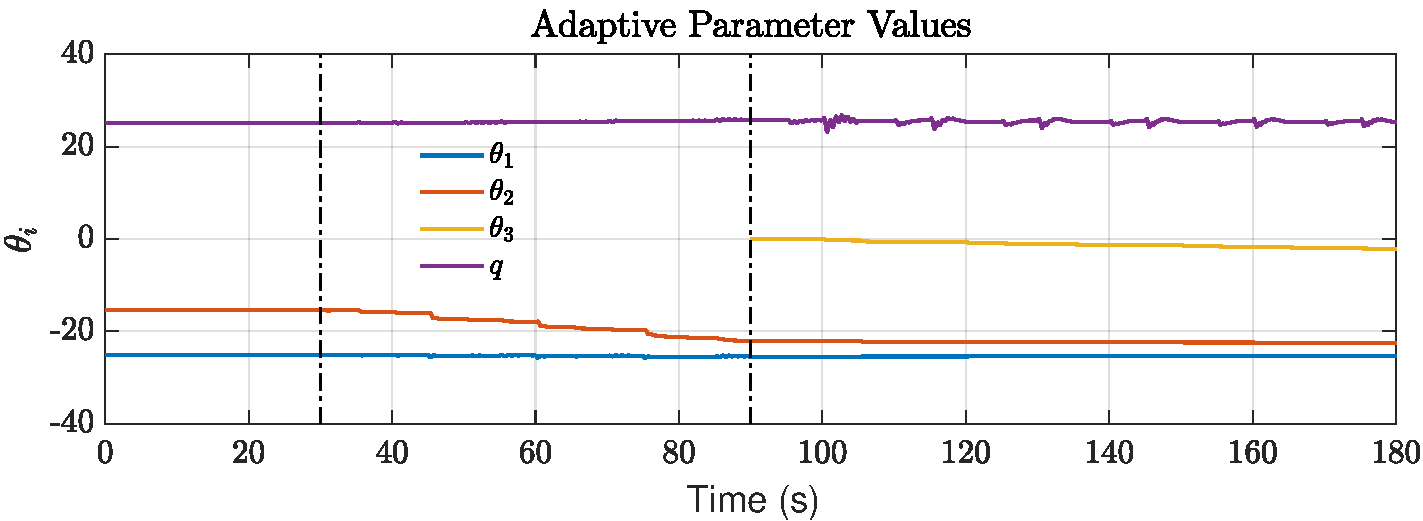
\includegraphics[width=\columnwidth]{theta_delay_v2.pdf}
	\caption{Del-AR simulation: Adaptive feedback gains under nominal operation ($t \leq t_1^*$), after abrupt addition of a time delay ($t_1^* < t \leq t_2^*$), and after a corrective action ($t > t_2^*$)}
	\label{fig:theta_d}
\end{figure}

\begin{figure}[h!]
	\centering
	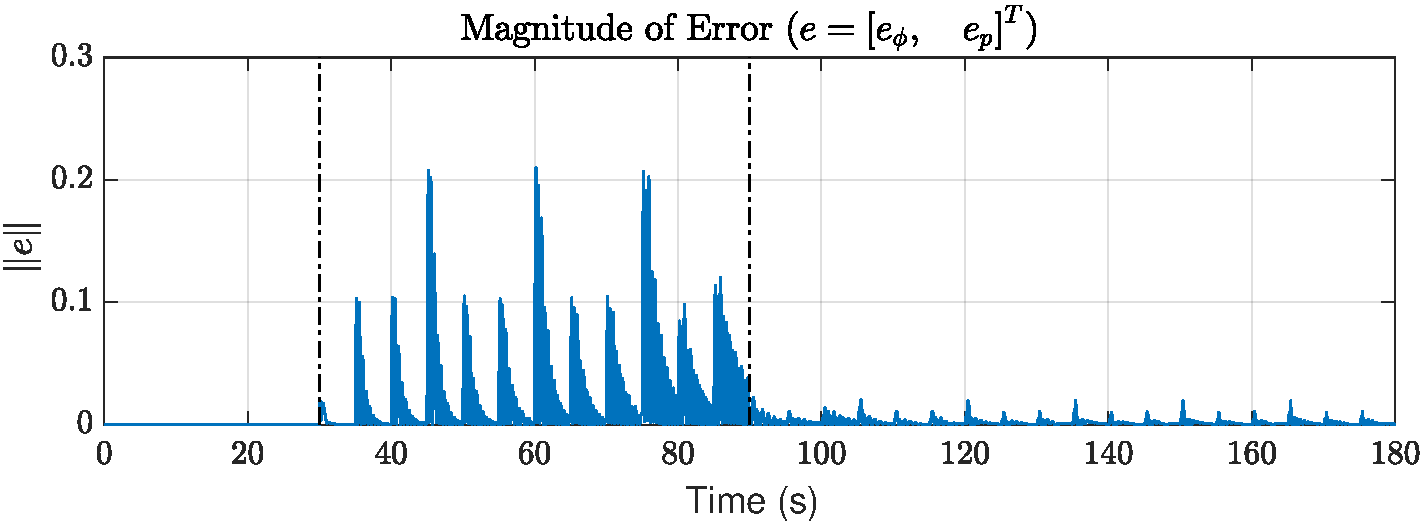
\includegraphics[width=\columnwidth]{e_delay_v2.pdf}
	\caption{Del-AR simulation: Tracking error $\|e\|$ under nominal operation ($t \leq t_1^*$), after abrupt addition of a time delay ($t_1^* < t \leq t_2^*$), and after a corrective action ($t > t_2^*$)}
	\label{fig:error_d}
\end{figure}

The resulting responses of the shared controller are shown in Figures \ref{fig:command_and_output_d}, \ref{fig:theta_d}, and \ref{fig:error_d}. From these results, we see that the adaptive controller with two feedback parameters has trouble tracking the commanded bank angle after the introduction of an anomaly, but the addition of a third feedback parameter ($\hat{\dot{p}}$) and a corresponding increase in the dimension of the reference model allows the controller to recover a reasonable tracking performance. It is worth noting that the model-following error does not converge to zero even with the recovery adaptive controller given by (\ref{eqn:control_law}), (\ref{eqn:thetadot_projection}), (\ref{eqn:qdot_projection}), and (\ref{eqn:rm_3}), because of the time delay approximation. 

The transfer functions used to generate step response plots in Figure \ref{fig:step_delay} use (\ref{eqn:theta_bar}) and (\ref{eqn:q_bar}) for average parameter values. Although the step response characteristics of Post-Correction differ more from nominal operation compared to the case of a change in actuator dynamics, the closed-loop response of Post-Correction is significantly more satisfactory than Post-Anomaly.

% TODO use ANOM-2 or something in captions
\begin{figure}[h!]
	\centering
	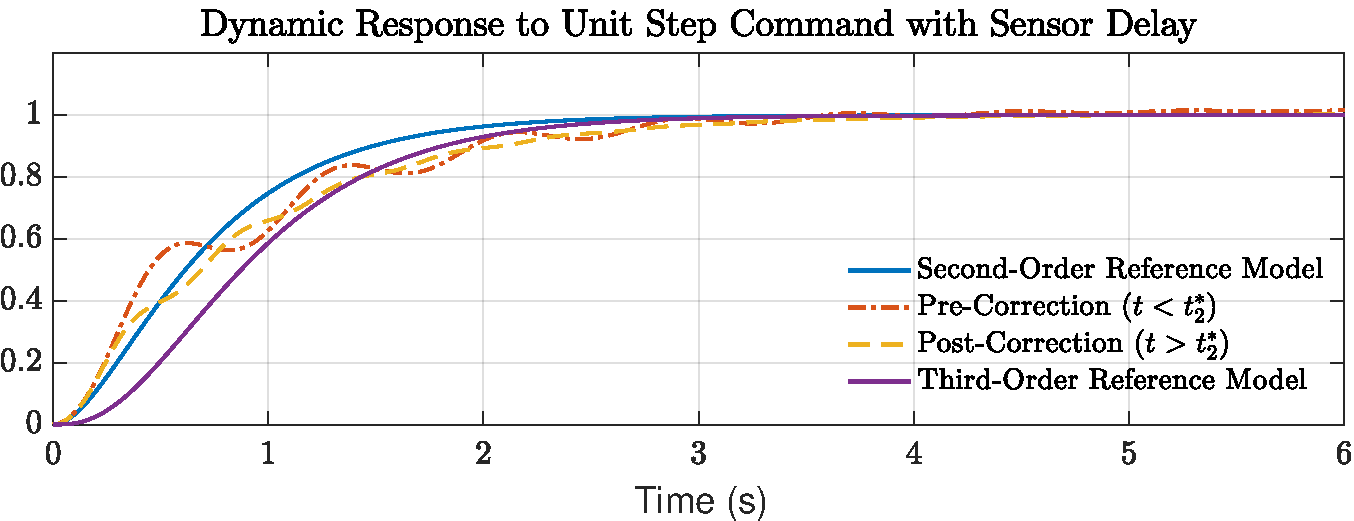
\includegraphics[width=\columnwidth]{step_delay_v2.pdf}
	\caption{Del-AR analysis: Unit step responses for closed-loop transfer functions at different stages of simulation, demonstrating performance improvement after corrective action}
	\label{fig:step_delay}
\end{figure}

One can compare this successful shared control response to an anomaly which introduced latency into sensor measurements against a passive response, in which the human pilot takes no action. In this case, the nominal adaptive controller retains responsibility for command tracking and regulation, which leads to structural failure at $t_3^* = 107$s. Command tracking, and eventual failure, in a simulation of this passive response is displayed in Fig. \ref{fig:command_and_output_d_fail}. It is noted that a shared control response with $t_2^* < t_3^*$ will lead to recovery of closed-loop tracking performance. 

% TODO did i introduce t_3^* earlier in SISO context?
\begin{figure}[h!]
	\centering
	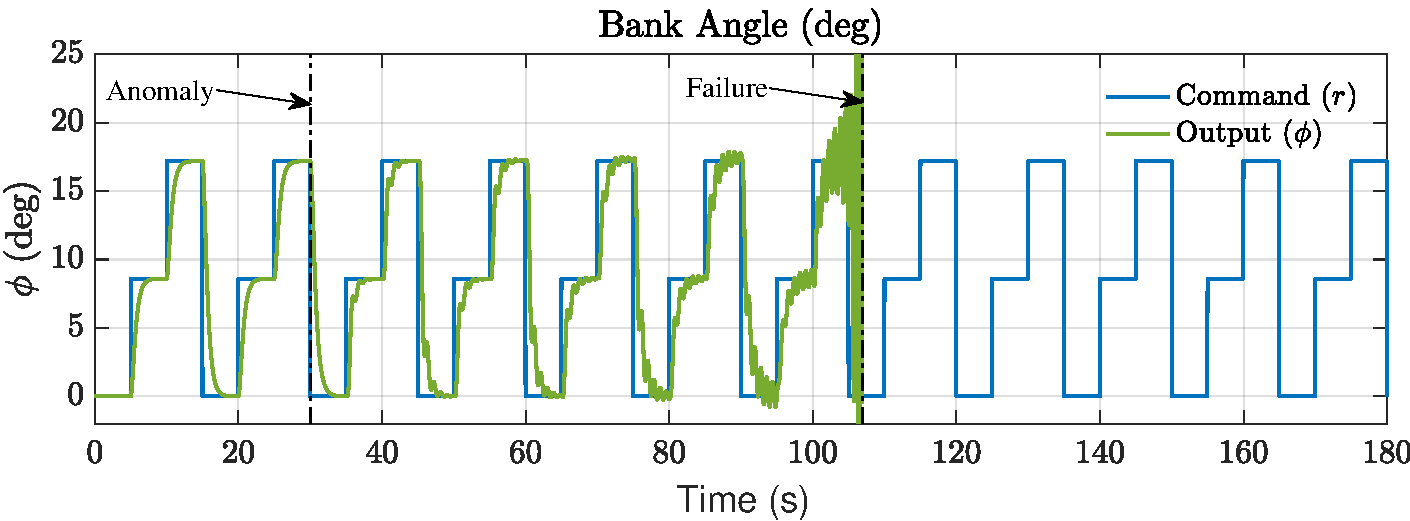
\includegraphics[width=\columnwidth]{phi_delay_failure.pdf}
	\caption{Del-AR-P simulation (passive anomaly response): The vehicle loses closed-loop stability following the anomaly when the shared control response is not implemented, and failure occurs at $t = t_3^*$}
	\label{fig:command_and_output_d_fail}
\end{figure}

\clearpage

\section{MIMO Output Feedback and Remote Pilot}
The shared control solution introduced in Chapter \ref{ch:mimo_shared_ctrl} is applied to the problem introduced in Section \ref{sec:mimo_problem} on a high altitude, long endurance (HALE) very flexible aircraft (VFA) model. HALE aerial platforms, such as the solar-electric NASA/AeroVironment Helios and Facebook Aquila, have unique design considerations to satisfy goals of uninterrupted weeks- or months-long operation. To reduce power draw, HALE aircraft designs save mass by allowing wings to bend, and may be classified as very flexible aircraft (VFA). Compared to typical fixed-wing aircraft, these aircraft operate at low speed, and may use low-bandwidth actuators which must be accounted for in control design. HALE VFA platforms are likely to have significant modeling uncertainties and online variation in dynamics due to flexible effects and degradation over long-term operation. It is assumed that these vehicles are unmanned and that they require supervision from remote human operators as needed.

The aircraft model used in simulation, developed by \cite{gibson2011modeling} for longitudinal control design applications, is rendered in Figure \ref{fig:vfa} and described in Section \ref{subsec:vfa_model}. The results of numerical simulations on the control and anomaly recovery with this MIMO plant are then presented in Section \ref{subsec:sims}, comparing the shared anomaly response to alternative anomaly responses.

\subsection{HALE Aircraft Model}\label{subsec:vfa_model}
%HALE VFA.

\begin{figure}[htbp]
	\centering
	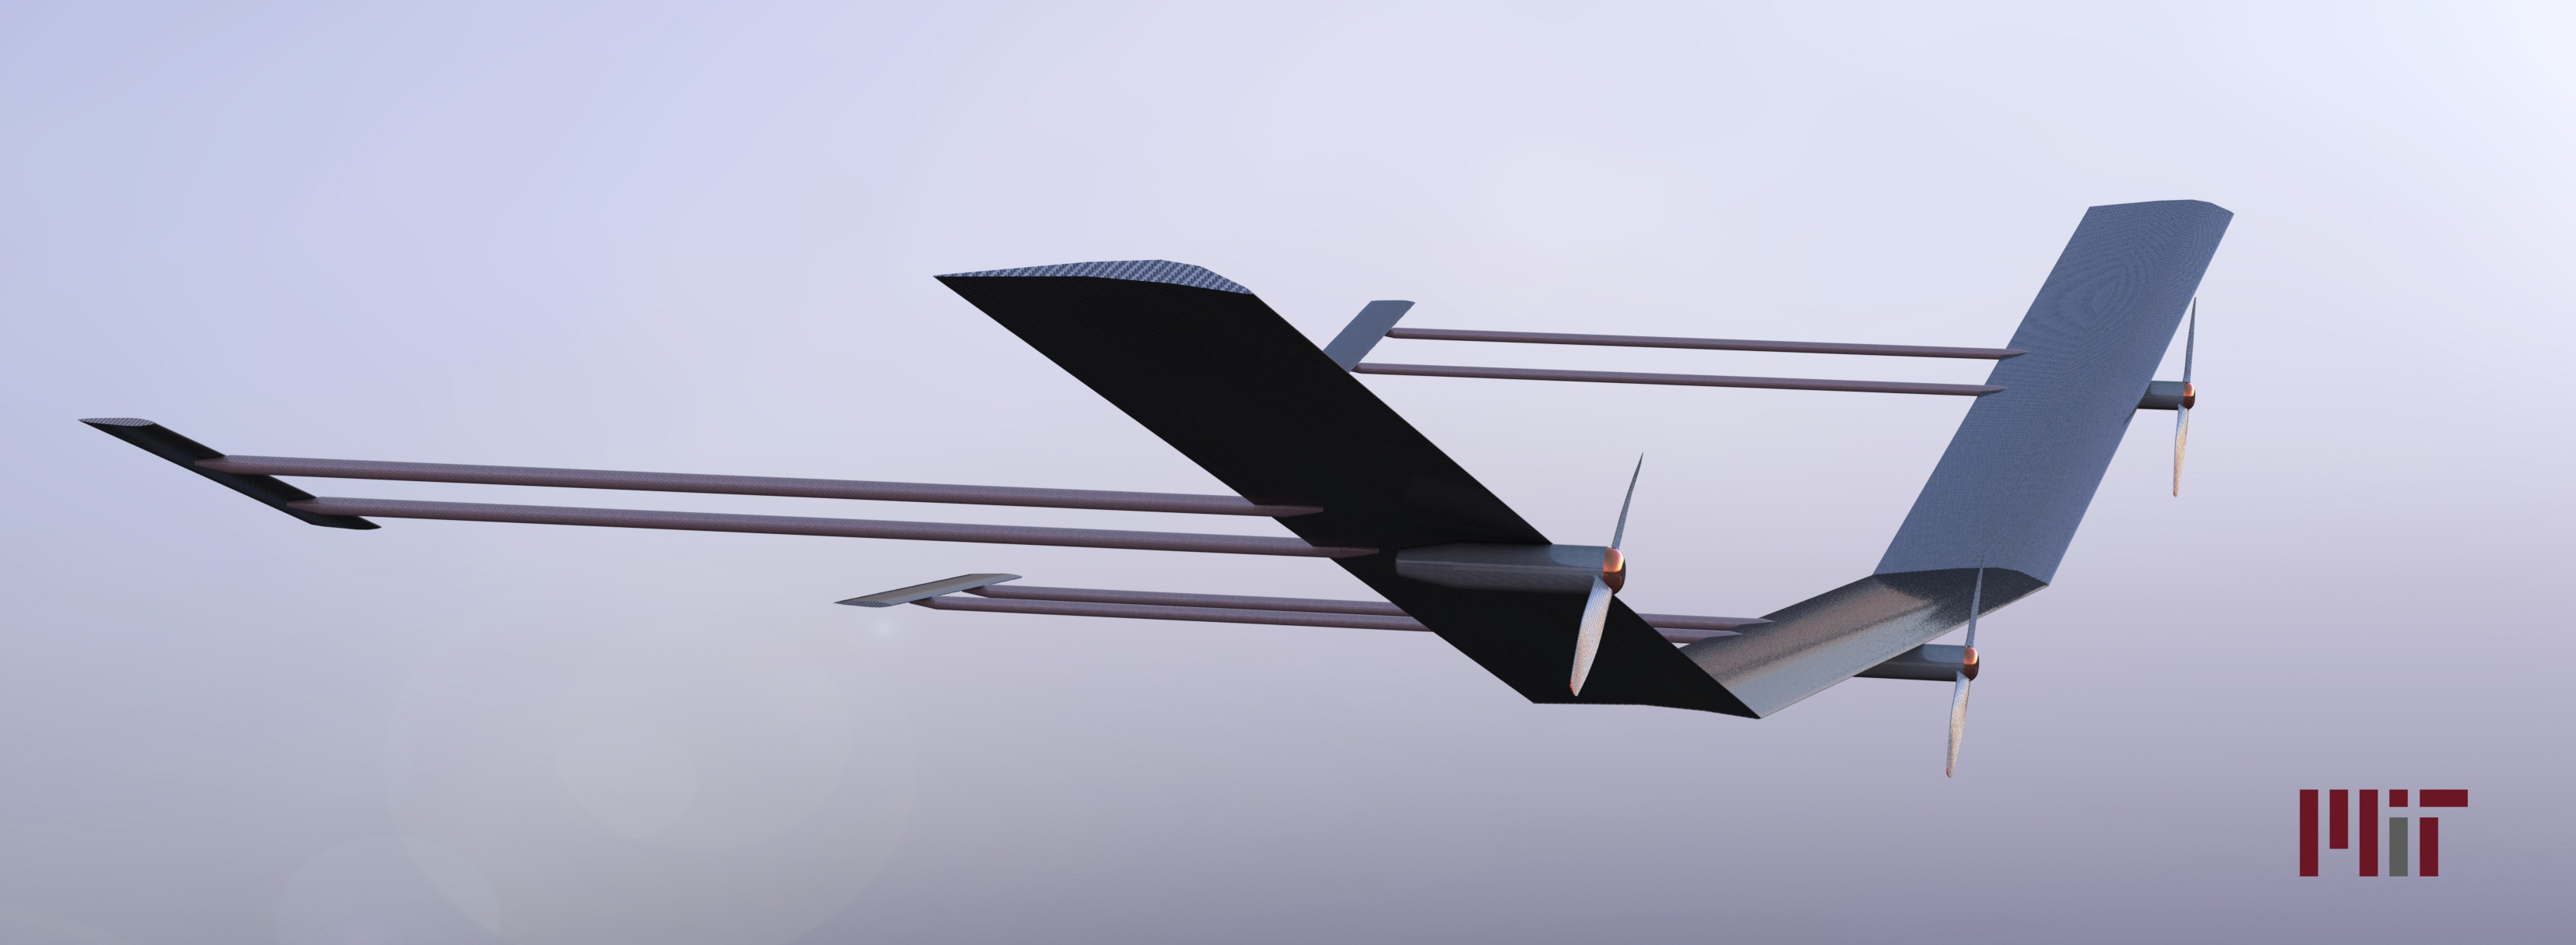
\includegraphics[width=0.95\columnwidth]{VFA_16.jpg}
	\caption{Rendering of very flexible aircraft model}
	\label{fig:vfa}
\end{figure}

The aircraft model represents the nonlinear longitudinal dynamics of a HALE VFA concept with three rigid lifting sections, hinged together such that the aircraft is able to bend at the joints of the three sections. The pitch mode dynamics of this nonlinear model is defined by the state vector
\begin{equation}
x_{\text{vfa}} = \begin{bmatrix}
~V~\\
\alpha \\
h \\
\theta \\
q\\
\eta\\
\dot{\eta}
\end{bmatrix} =
\begin{bmatrix}
	 $Airspeed (ft/s)$\\ $Angle of attack (rad)$\\ $Altitude (ft)$\\ $Pitch angle (rad)$\\ $Pitch rate (rad/s)$\\ $Dihedral (rad)$\\ $Dihedral rate (rad/s)$
\end{bmatrix}
\end{equation}
We linearize and trim the aircraft in straight and level flight using the inputs
\begin{equation}
	u_{\text{vfa}} = \begin{bmatrix}
\delta_{th} \\
\delta_{a,c} \\
\delta_{a,o} \\
\delta_{e,c} \\
\delta_{e,o} 
\end{bmatrix} = \begin{bmatrix}
		$Thrust (lbf)$\\
		$Center aileron (rad)$\\
		$Outer aileron (rad)$\\
		$Center elevator (rad)$\\
		$Outer elevator (rad)$
	\end{bmatrix}
\end{equation}
Assuming small deviations in altitude, the state vector corresponding to (\ref{eq:plant_dynamics}) is
\begin{equation}
	x_p = \begin{bmatrix}
V & \; \alpha & \; \theta & \; q & \; \eta & \; \dot{\eta}
\end{bmatrix}^T.
\end{equation}

We consider the control task of tracking commands for the dihedral angle and vertical acceleration, using control inputs $\delta_{a,o}$ and $\delta_{e,c}$ only, so the vector $u_p$ in (\ref{eq:plant_dynamics}) is
\begin{equation}
	u_p = \begin{bmatrix}
\delta_{a,o} & \; \delta_{e,c}
\end{bmatrix}^T.
\end{equation}

Regulation of the dihedral angle is desired, as a large dihedral angle is inefficient for lift generation and introduces instability in the open-loop dynamics, while a small dihedral angle will require more control effort to hold, increasing drag and power requirements and imparting twisting moments on the aircraft. 

The measurements available for control design are the pitch rate, dihedral angle, and vertical acceleration, leading to plant outputs
\begin{equation}
\begin{aligned}
y_p =& \, \Big[\; q \; \Big] \;= \Big[\: \text{Pitch rate (rad/s)} \:\Big] \\
z_p =& \begin{bmatrix}
\eta \\
A_z
\end{bmatrix} =\begin{bmatrix}
	$Dihedral angle (rad)$\\
	$Vertical acceleration (ft/s)$
\end{bmatrix}		
\end{aligned}
\end{equation}
and the outputs for the augmented plant (\ref{eq:augmented_plant}),
\begin{equation}
y = \begin{bmatrix}
	q \\ \int{z_p - z_{cmd}}
\end{bmatrix}, \quad z = z_p.
\end{equation}

For numerical simulations, the VFA model is trimmed at an airspeed of $68$ ft/s, altitude of 40,000 ft, $2.8^\circ$ angle of attack and pitch angle (level flight), and dihedral angles ranging from $0$ to $20^\circ$ in $1^\circ$ increments. Figure \ref{fig:trim-poles} shows pole locations of the linearized plant for different dihedral angles, and Figure \ref{fig:trim-poles-zoom} shows instability of the linearized plant when trimmed above $11^\circ$ dihedral. Figure \ref{fig:trim-inputs} shows the thrust and control surface deflections for the trimmed VFA model over a range of dihedral angles.

\begin{figure}[htbp]
	\centering
	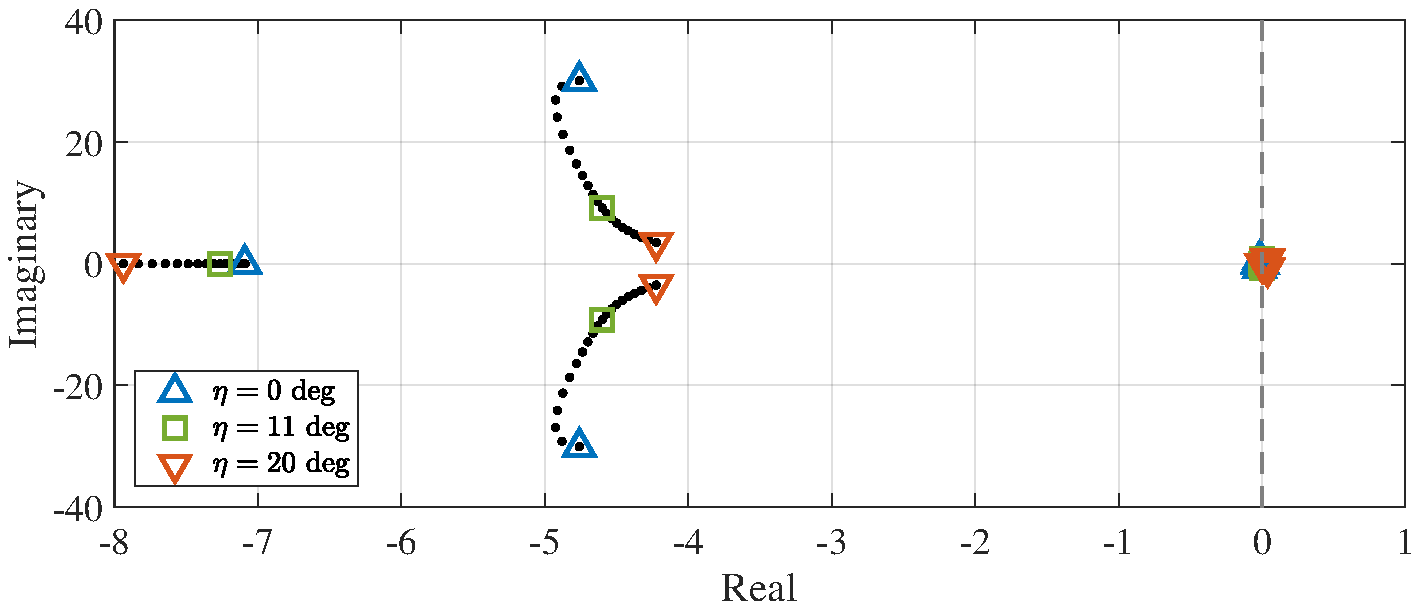
\includegraphics[width=0.95\columnwidth]{trim-poles-2.pdf}
	\caption{Poles of linearized system for different dihedral angles}
	\label{fig:trim-poles}
\end{figure}

\begin{figure}[htbp]
	\centering
	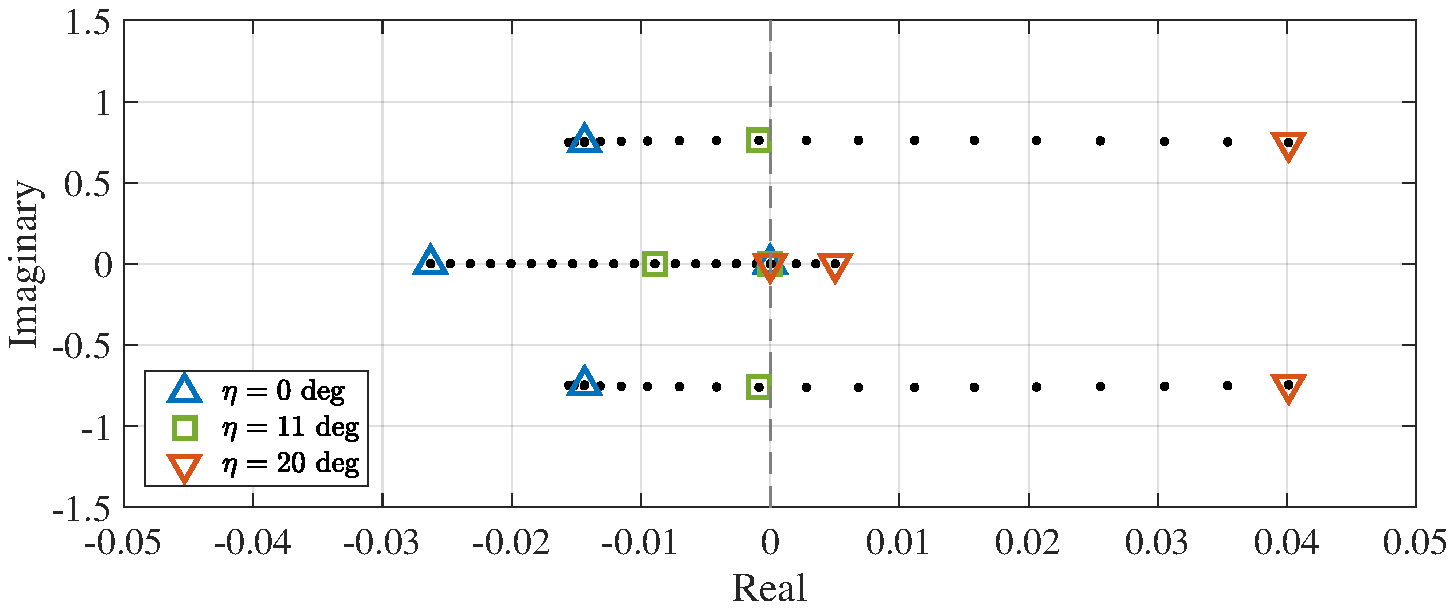
\includegraphics[width=0.95\columnwidth]{trim-poles-zoom-2.pdf}
	\caption{Dominant poles of linearized system, which move into the right-half complex plane when $\eta > 11^\circ$}
	\label{fig:trim-poles-zoom}
\end{figure}

\begin{figure}[htbp]
	\centering
	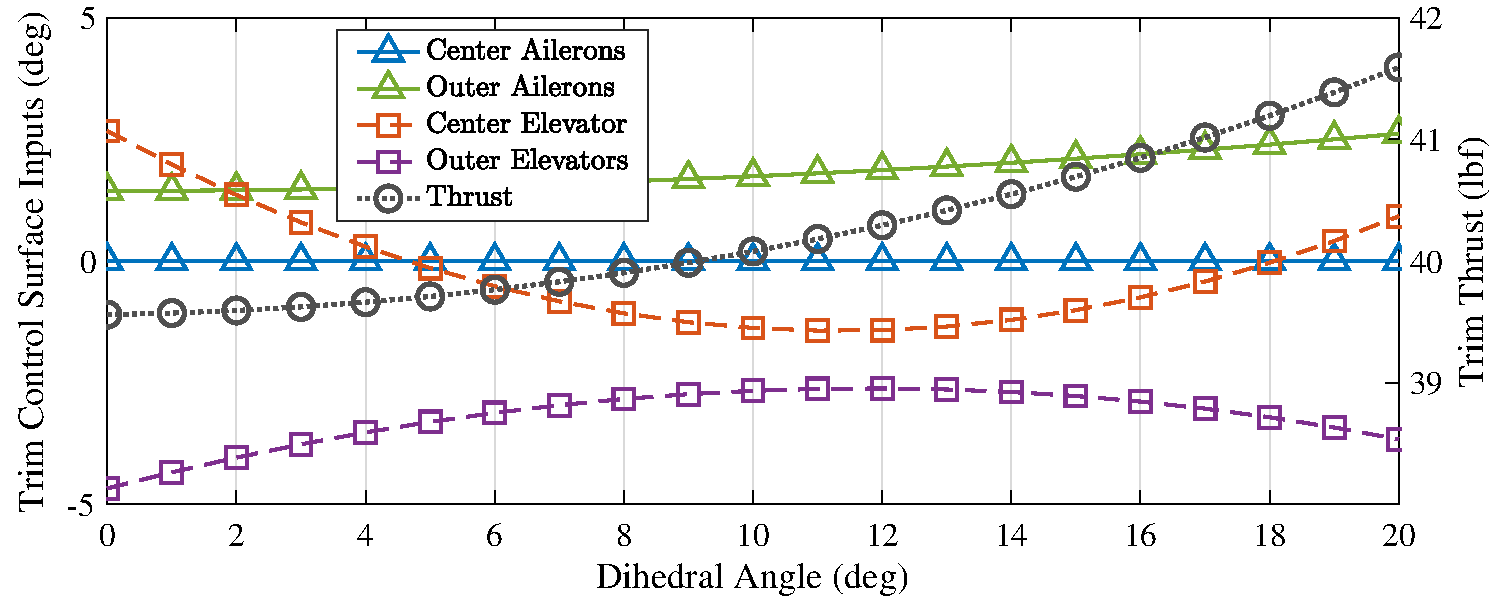
\includegraphics[width=0.95\columnwidth]{trim-inputs-3.pdf}
	\caption{Actuator trim at different dihedral angles}
	\label{fig:trim-inputs}
\end{figure}

The plant is augmented with a linear actuator model corresponding to (\ref{eq:first_order_act}) in the nominal case and (\ref{eq:second_order_act}) in the presence of anomalous dynamics. The vehicle simulation with first-order actuators (\ref{eq:first_order_act}) uses time constants $(\hat{\tau},\;\tau) = (0.5,\,2.0)$s in the control model and the actual plant, respectively, corresponding to
\begin{equation}
D_1 = 2 I_2, \quad \Theta_1 = -1.5 I_2 \label{eq:theta_1}
\end{equation}
where $\Theta_1$ is unknown for control design, and $I_2$ is the $2 \times 2$ identity matrix. 

Simulation of the anomalous dynamics (\ref{eq:second_order_act}) uses second-order actuators with cutoff frequencies $(\hat{\omega}_c,\; \omega_c) = (2.0 ,\; 1.0)$ rad/s and damping ratios $(\hat{\zeta},\; \zeta) = (0.7,\; 0.8)$ in the control model and actual plant, respectively, corresponding to
\begin{equation}
\begin{bmatrix}
	D_1 \\ D_2
\end{bmatrix} = \begin{bmatrix}
	4 I_2 \\ 2.8 I_2
\end{bmatrix}, \quad \begin{bmatrix}
	\Theta_1 \\ \Theta_2 
\end{bmatrix} = \begin{bmatrix}
	-3.75 I_2 \\ -2 I_2
\end{bmatrix}
\end{equation}
where $\Theta_1$ and $\Theta_2$ are unknown for control design. Matrices $\Theta_p$ and $\Lambda_p$ used in simulation represent modeling errors that are assumed to be caused by linearization of the VFA model at an incorrect dihedral angle, and an 80\% reduction in actuator effectiveness, respectively, and are given by
\begin{equation}
\begin{gathered}
\Theta_{p}^{T}=\begin{bmatrix}
0.6 & -4.52 & \; 0 & \hfill 0.05 & \hfill 0.41 & \hfill 1.47\\
0.1 & \hfill 1.83 & \; 0 & -0.02 & -0.35 & -0.59
\end{bmatrix}\\ \Lambda = 0.2 I_2. \end{gathered} \label{eq:theta_p}
\end{equation}
Both the nominal and recovery adaptive controllers utilize a number of free design parameters, including LQR weight matrices and adaptation rates. These parameters are tabulated in Appendix \ref{app:params}.


\subsection{Numerical Simulations and Results} \label{subsec:sims}
We begin by simulating the HALE VFA under nominal autonomous control, responding to step inputs in commands for the dihedral angle and vertical acceleration, with the following three variants.
\begin{description}
	\item[Nom-1] Command tracking using baseline RSLQR controller without uncertainty in control model ($\Theta_p = 0$, $\Lambda_p = 0$, $\Theta_1 = 0$)
	\item[Nom-2] Command tracking using baseline RSLQR controller with uncertainty in control model ($\Theta_1$ in (\ref{eq:theta_1}); $\Theta_p$, $\Lambda_p$ in (\ref{eq:theta_p}))
	\item[Nom-3] Command tracking using [baseline RSLQR + adaptive] controller with uncertainty in control model ($\Theta_1$ in (\ref{eq:theta_1}); $\Theta_p$, $\Lambda_p$ in (\ref{eq:theta_p}))
\end{description}

\begin{figure}[htbp]
	\centering
	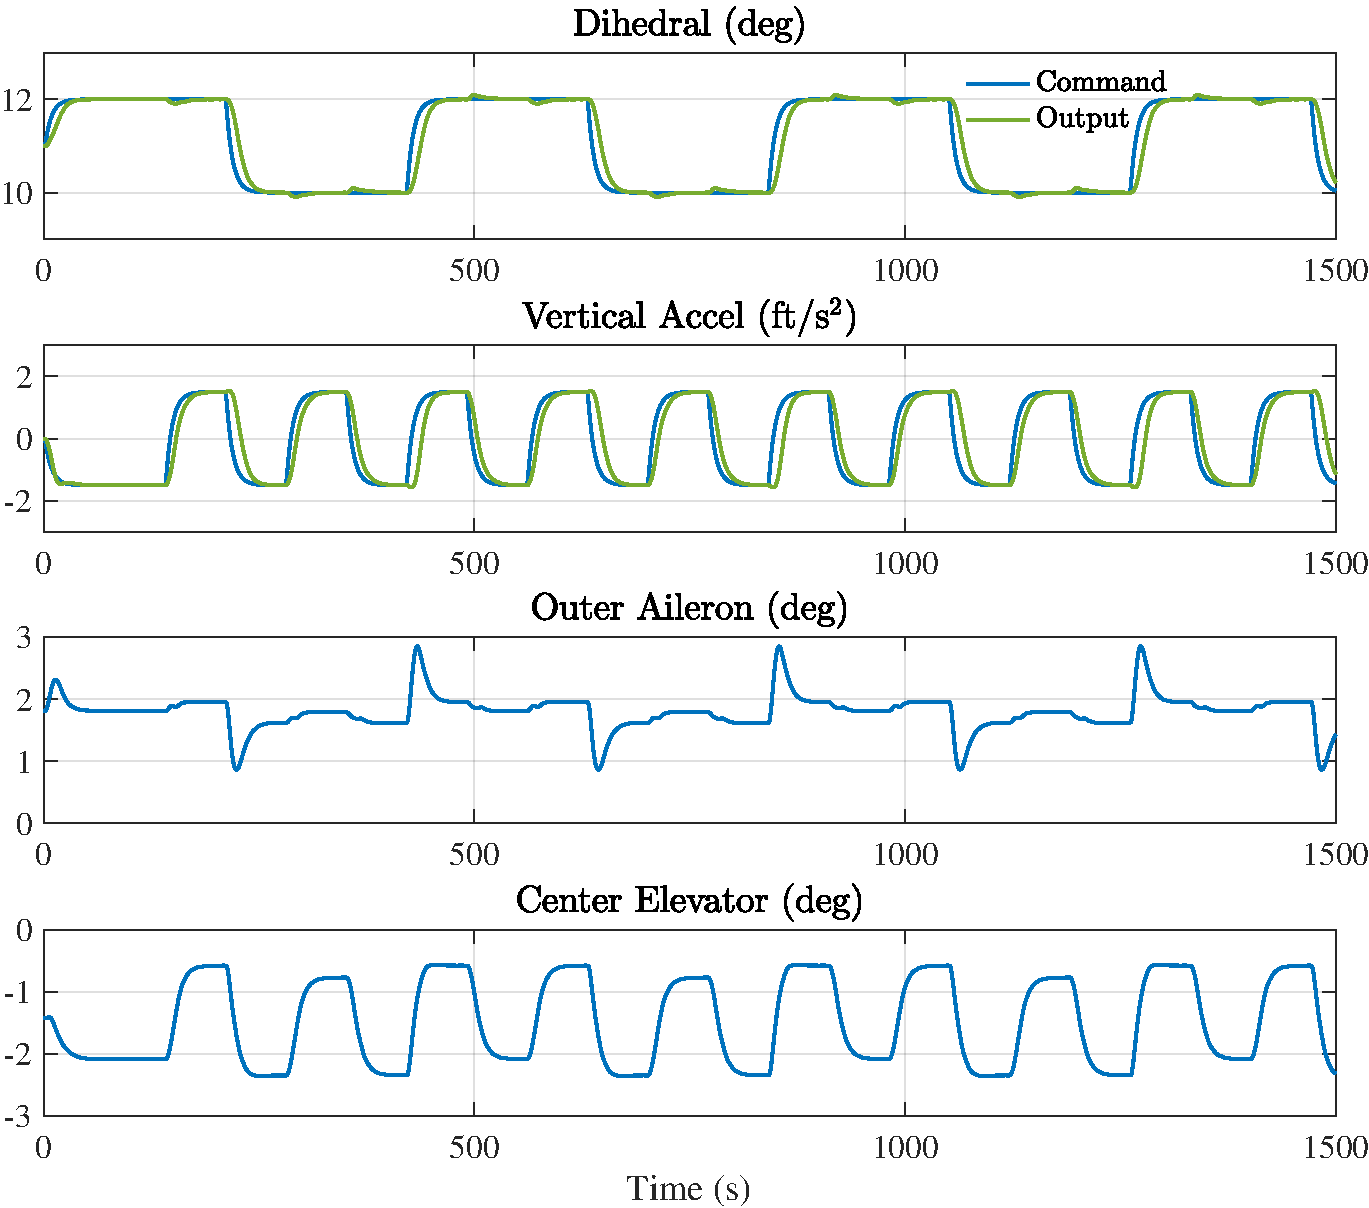
\includegraphics[width=\columnwidth]{nom1.pdf}
	\caption{Nom-1 simulation: Control of longitudinal dynamics of VFA model using RSLQR, with no uncertainty in the control model}
	\label{fig:nom1}
\end{figure}

\begin{figure}[htbp]
	\centering
	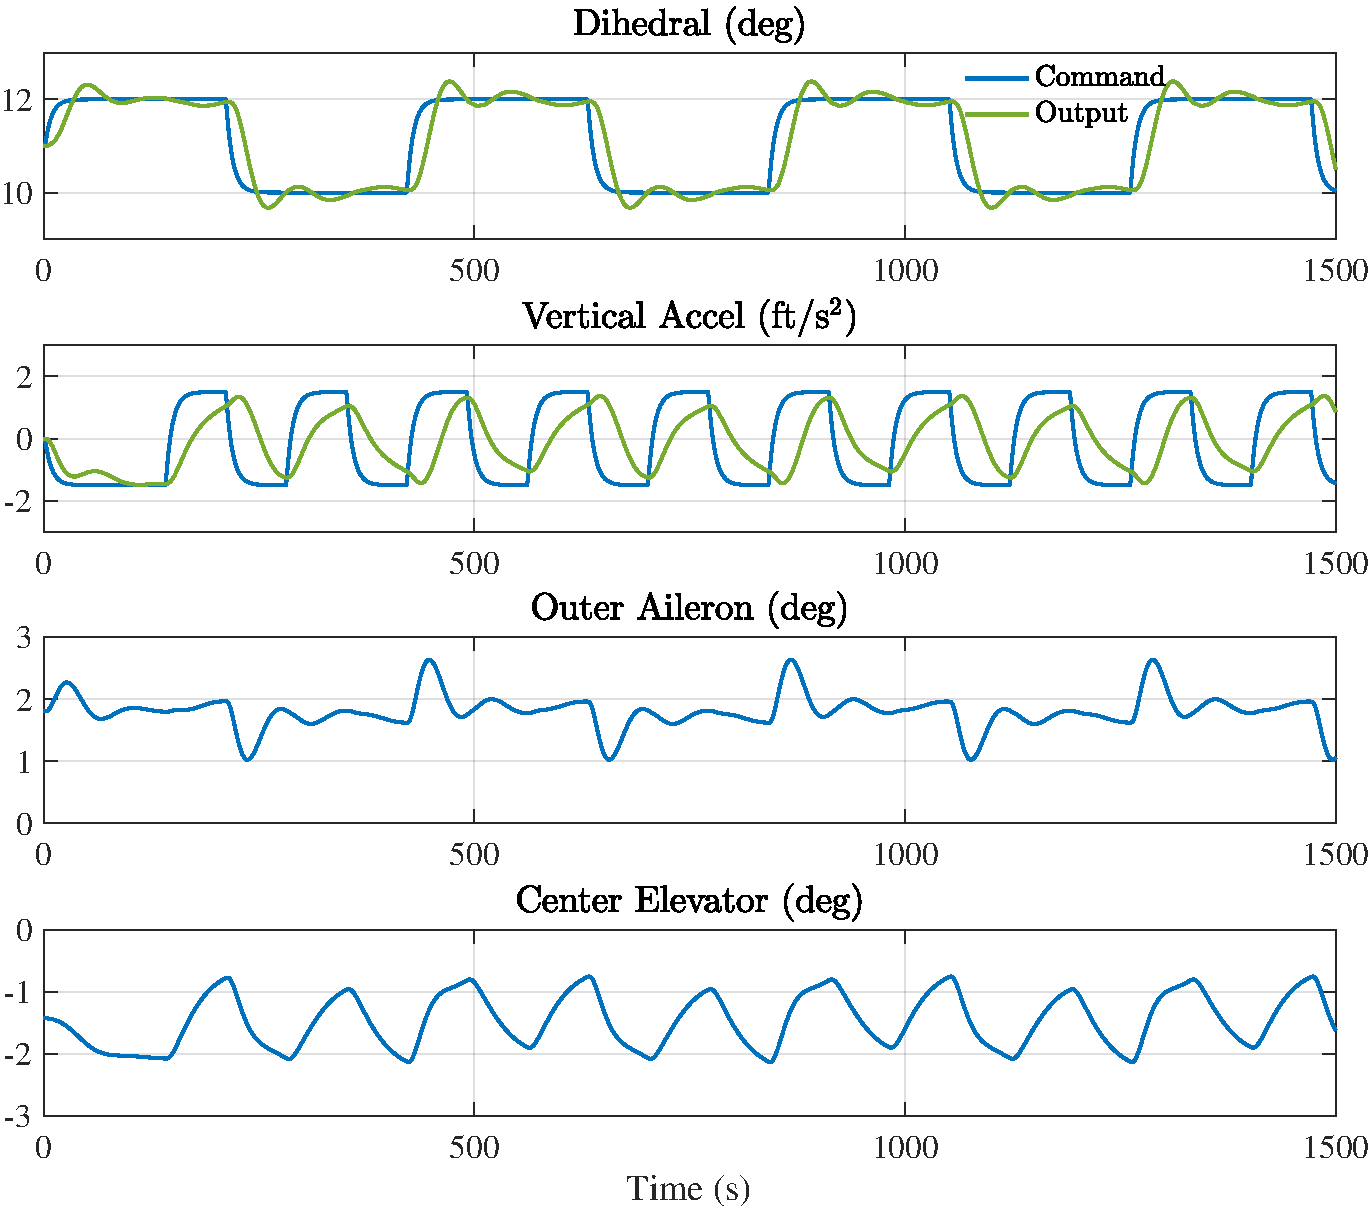
\includegraphics[width=\columnwidth]{nom2.pdf}
	\caption{Nom-2 simulation: Control of longitudinal dynamics of VFA model using RSLQR, with uncertainties $\Theta_p$, $\Lambda_p$, and $\Theta_1$}
	\label{fig:nom2}
\end{figure}

\begin{figure}[htbp]
	\centering
	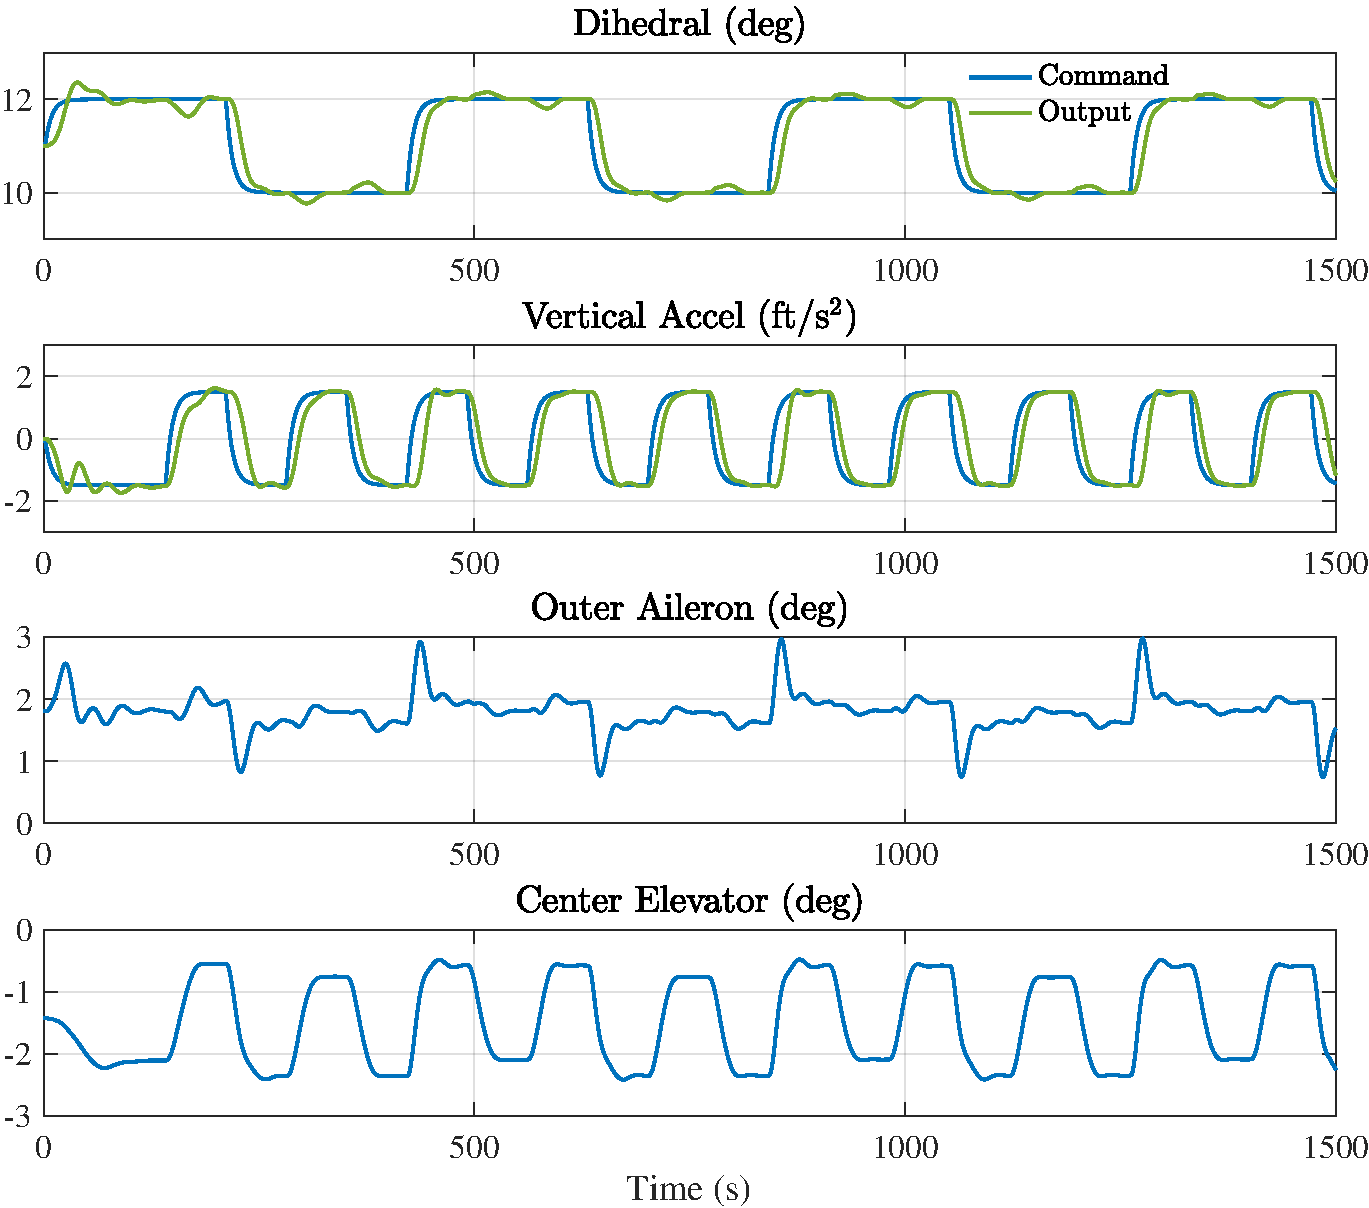
\includegraphics[width=\columnwidth]{nom3.pdf}
	\caption{Nom-3 simulation: Control of longitudinal dynamics of VFA model using RSLQR + adaptive control, with uncertainties $\Theta_p$, $\Lambda_p$, and $\Theta_1$}
	\label{fig:nom3}
\end{figure}

These simulations, presented in Figs. \ref{fig:nom1}, \ref{fig:nom2}, and \ref{fig:nom3} respectively, show how the adaptive controller with output feedback described in (\ref{eq:rd2-b1a})--(\ref{eq:rd2-adaptation}) is able to recover the desired closed-loop performance with uncertainty in plant and actuator parameters. With the baseline RSLQR controller only, the system suffers degraded command tracking performance in the presence of uncertainty (Fig. \ref{fig:nom2}), especially for vertical acceleration tracking.

In what follows, we simulate the introduction of an anomaly into the dynamics, causing the vehicle's actuators to change abruptly from the uncertain first-order dynamics (\ref{eq:first_order_act}) to the uncertain second-order dynamics (\ref{eq:second_order_act}) at $t_1^* = 600s$. We consider three responses to the anomaly.
\begin{description}
	\item[AR-1 (Passive)] The nominal adaptive autopilot retains control without intervention from the remote human supervisor
	\item[AR-2 (Manual)] The human operator takes over manual control of the affected vehicle
	\item[AR-3 (Shared)] Responsibilities are shared between the human pilot and autopilot as described in Chapter \ref{ch:mimo_shared_ctrl}
\end{description}

In these simulations, the vehicle operates in nominal operation with the [RSLQR + adaptive] control design for $0 \leq t < t_1^*$. At $t_1^* = 600 s$, the vehicle's actuators change from first-order (\ref{eq:first_order_act}) to second-order (\ref{eq:second_order_act}). Figs. \ref{fig:ar1} to \ref{fig:ar1-err} show the result of a passive response (AR-1) in which the human operator ignores vehicle performance degradation and allows the adaptive controller to continue operating on the plant with severely anomalous dynamics. The closed-loop system loses stability, leading to oscillations in vehicle output and eventual structural failure of the VFA at $t_3^* = 960s$, 6 minutes after the introduction of second-order actuator dynamics. It is worth noting the rapid increase in magnitude of the adaptive parameters and the magnitudes of both tracking and measurement output error signals after the introduction of anomalous dynamics. For comparison to a baseline without adaptive control, a passive response using only the RSLQR controller (denoted AR-1-LQR) leads to structural failure following the anomaly, at $t = 1240s$, as shown in Fig. \ref{fig:ar-lqr}.

\begin{figure}[htbp]
	\centering
	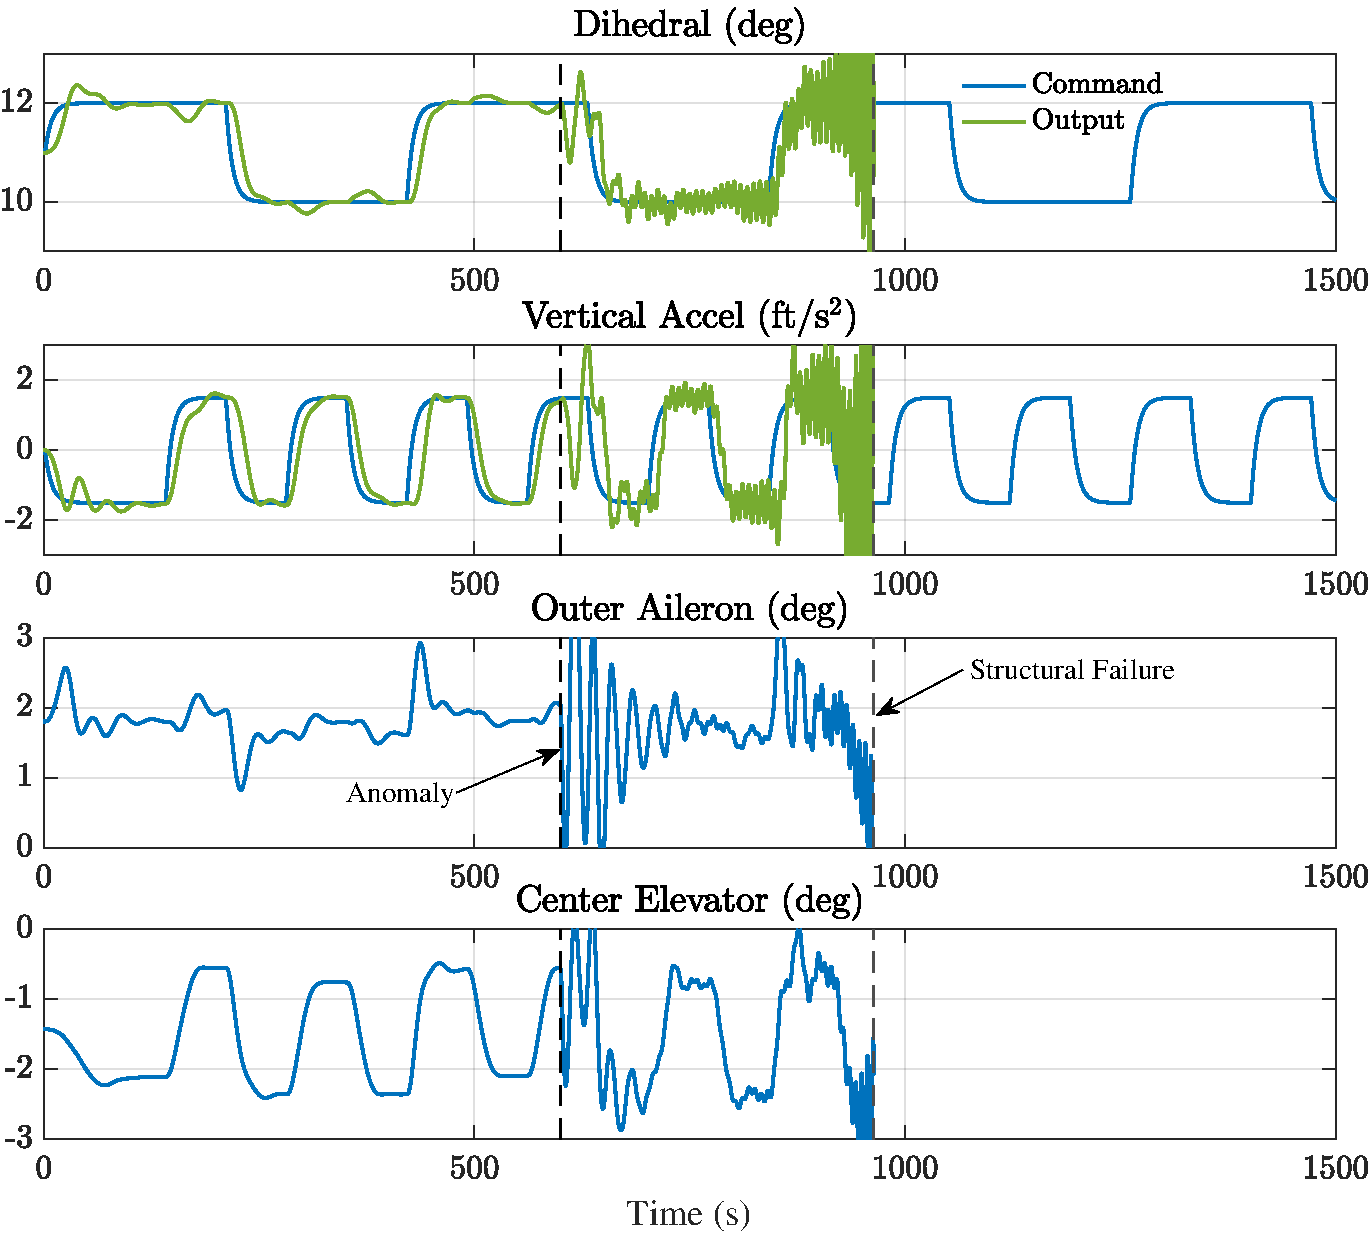
\includegraphics[width=\columnwidth]{ar1.pdf}
	\caption{AR-1 simulation: Passive response to dynamical anomaly results in structural failure after 6 minutes}
	\label{fig:ar1}
\end{figure}

\begin{figure}[htbp]
	\centering
	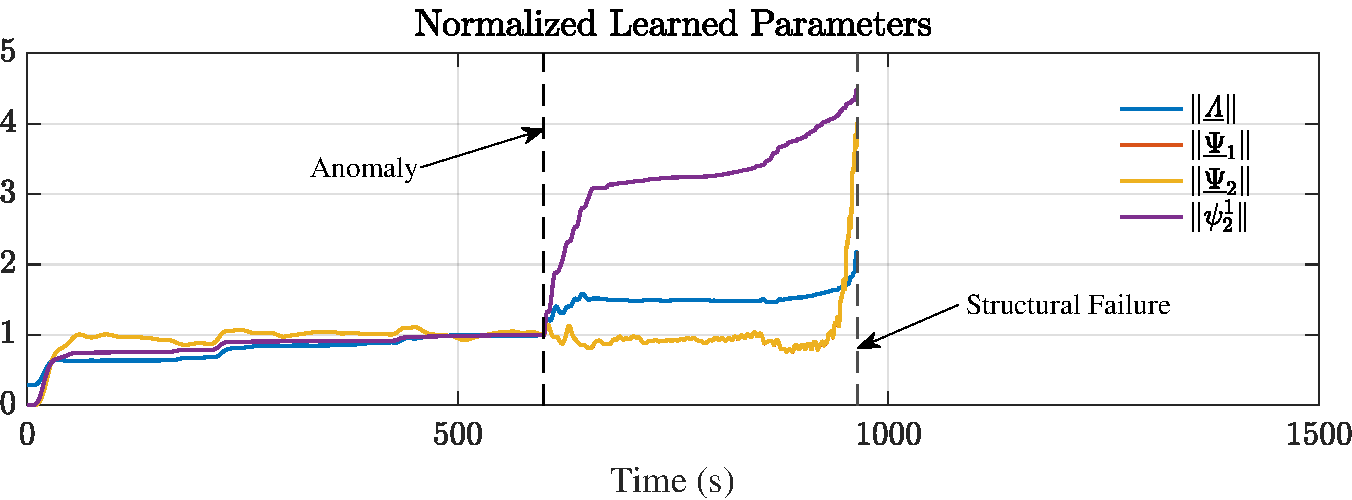
\includegraphics[width=\columnwidth]{ar1-params.pdf}
	\caption{AR-1 simulation: Adaptive parameters diverge as controller struggles to adapt to unmodeled dynamics}
	\label{fig:ar1-params}
\end{figure}

\begin{figure}[htbp]
	\centering
	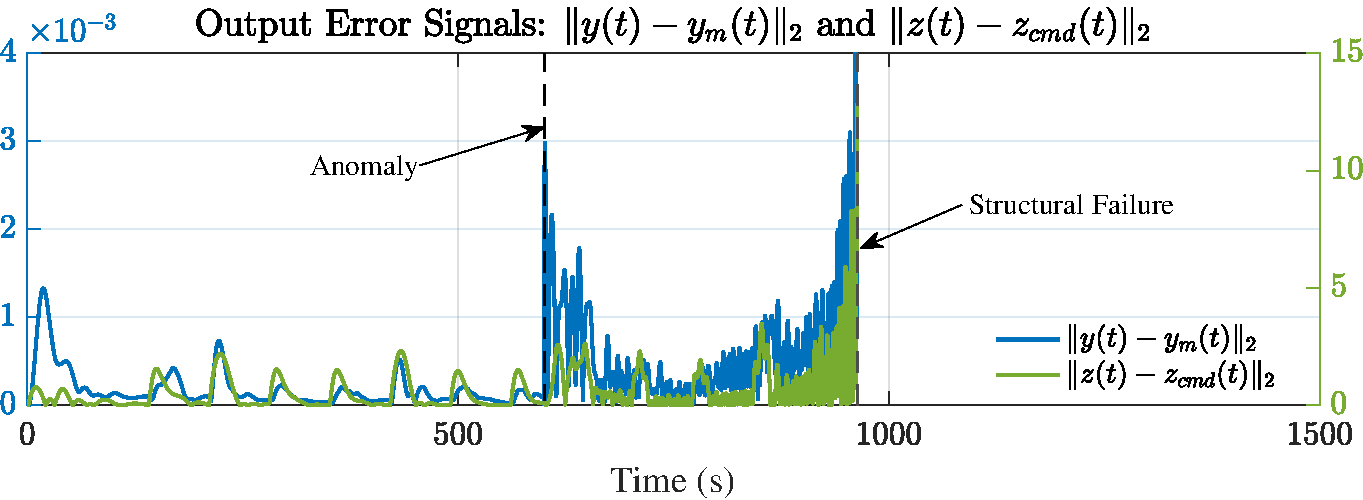
\includegraphics[width=\columnwidth]{ar1-err.pdf}
	\caption{AR-1 simulation: Model-following output error and command tracking error grow due to anomalous dynamics}
	\label{fig:ar1-err}
\end{figure}

\begin{figure}[htbp]
	\centering
	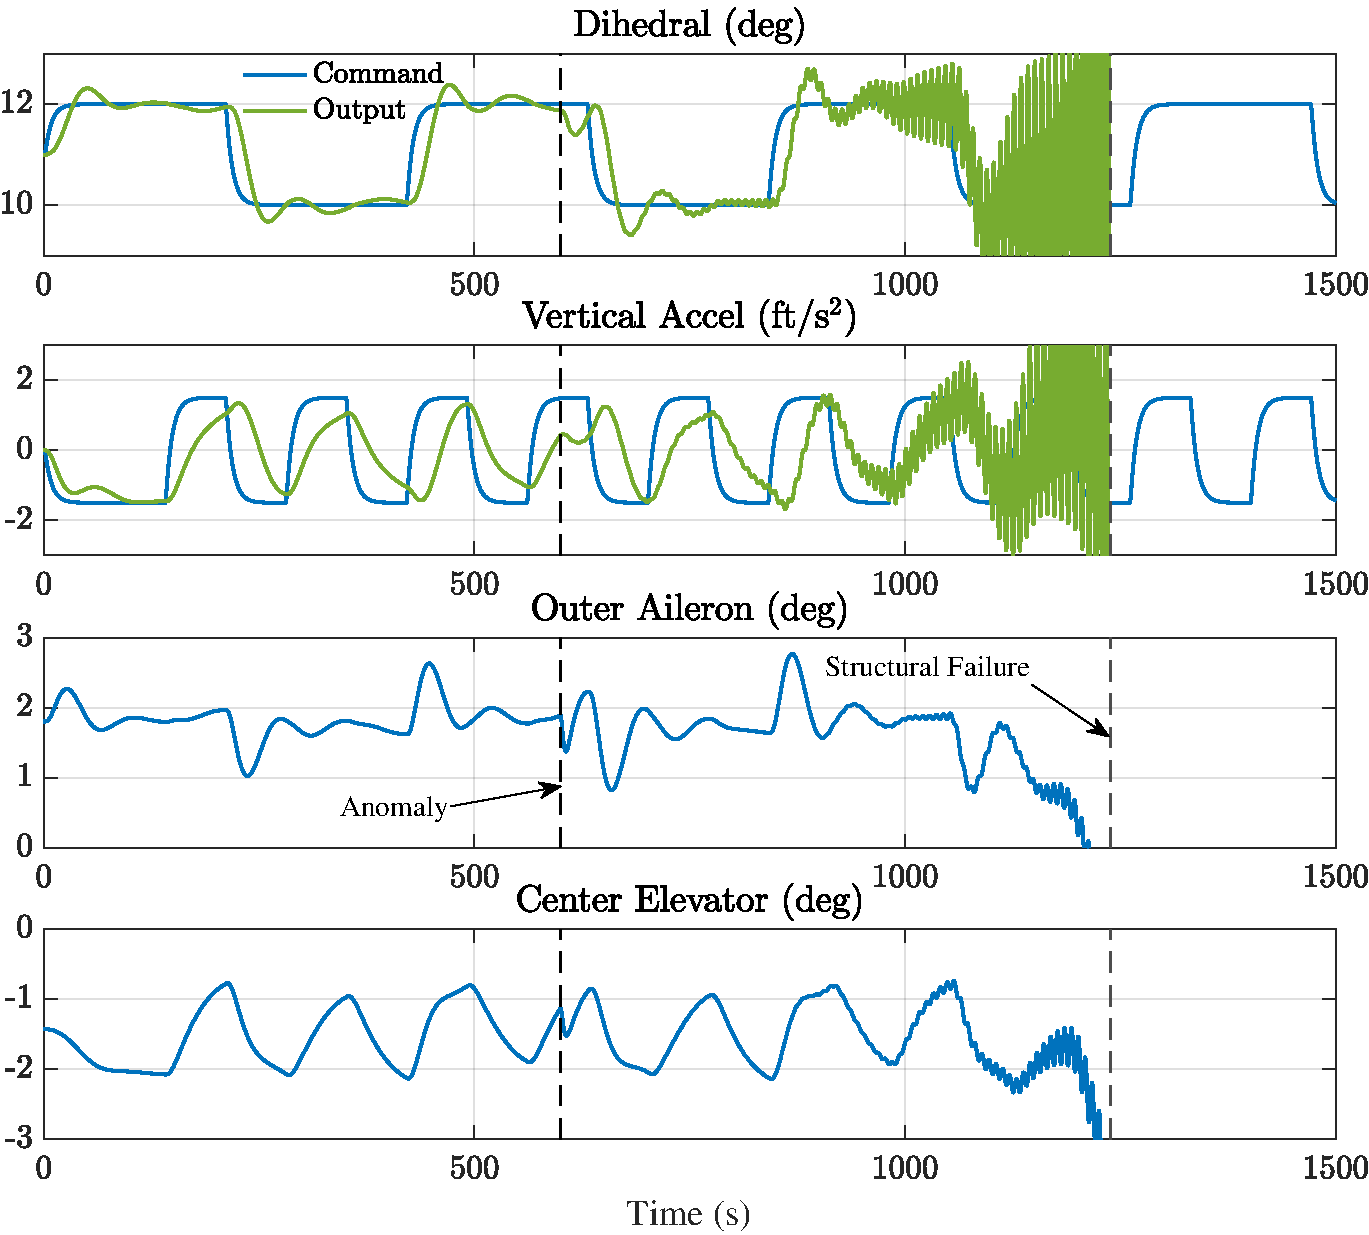
\includegraphics[width=\columnwidth]{ar-lqr.pdf}
	\caption{AR-1-LQR simulation: Passive response to dynamical anomaly using only baseline RSLQR control (no adaptive) also results in structural failure}
	\label{fig:ar-lqr}
\end{figure}

Numerical simulations of the AR-2 response (purely manual control) are not carried out, as they are not deterministic and require high-fidelity \textit{human-in-the-loop} experiments to characterize. The limitations of such a response -- in which the human operator's role changes suddenly from ``on-the-loop'' to ``in-the-loop'' with unfamiliar dynamics -- are discussed in the earlier sections of this thesis, and in references elsewhere (e.g. \cite{endsley1996automation}, \cite{hess2015modeling}).

Results of the AR-3 (shared control) anomaly response simulation are shown in Figs. \ref{fig:ar3-sim} to \ref{fig:ar3-err}. After the anomaly is introduced at $t_1^* = 600 s$, the nominal adaptive controller attempts to control the system whose dynamics are not fully accounted for in the control model. Simultaneously in the shared control framework, the human operator notices the anomalous closed-loop control behavior, and via an interface switches the controller to the higher relative degree design (\ref{eq:rd3-b1a})--(\ref{eq:rd3-adaptation-deriv}) t $t_2^* = 800 s$, which is the culmination of the human operator's action. For $t \geq t_2^*$, the vehicle remains under autonomous control with the recovery adaptive controller and is able to reestablish nominal command tracking performance and avert failure (which was assumed to occur at $t_3^* = 960 s$ with AR-1).

\begin{figure}[htbp]
	\centering
	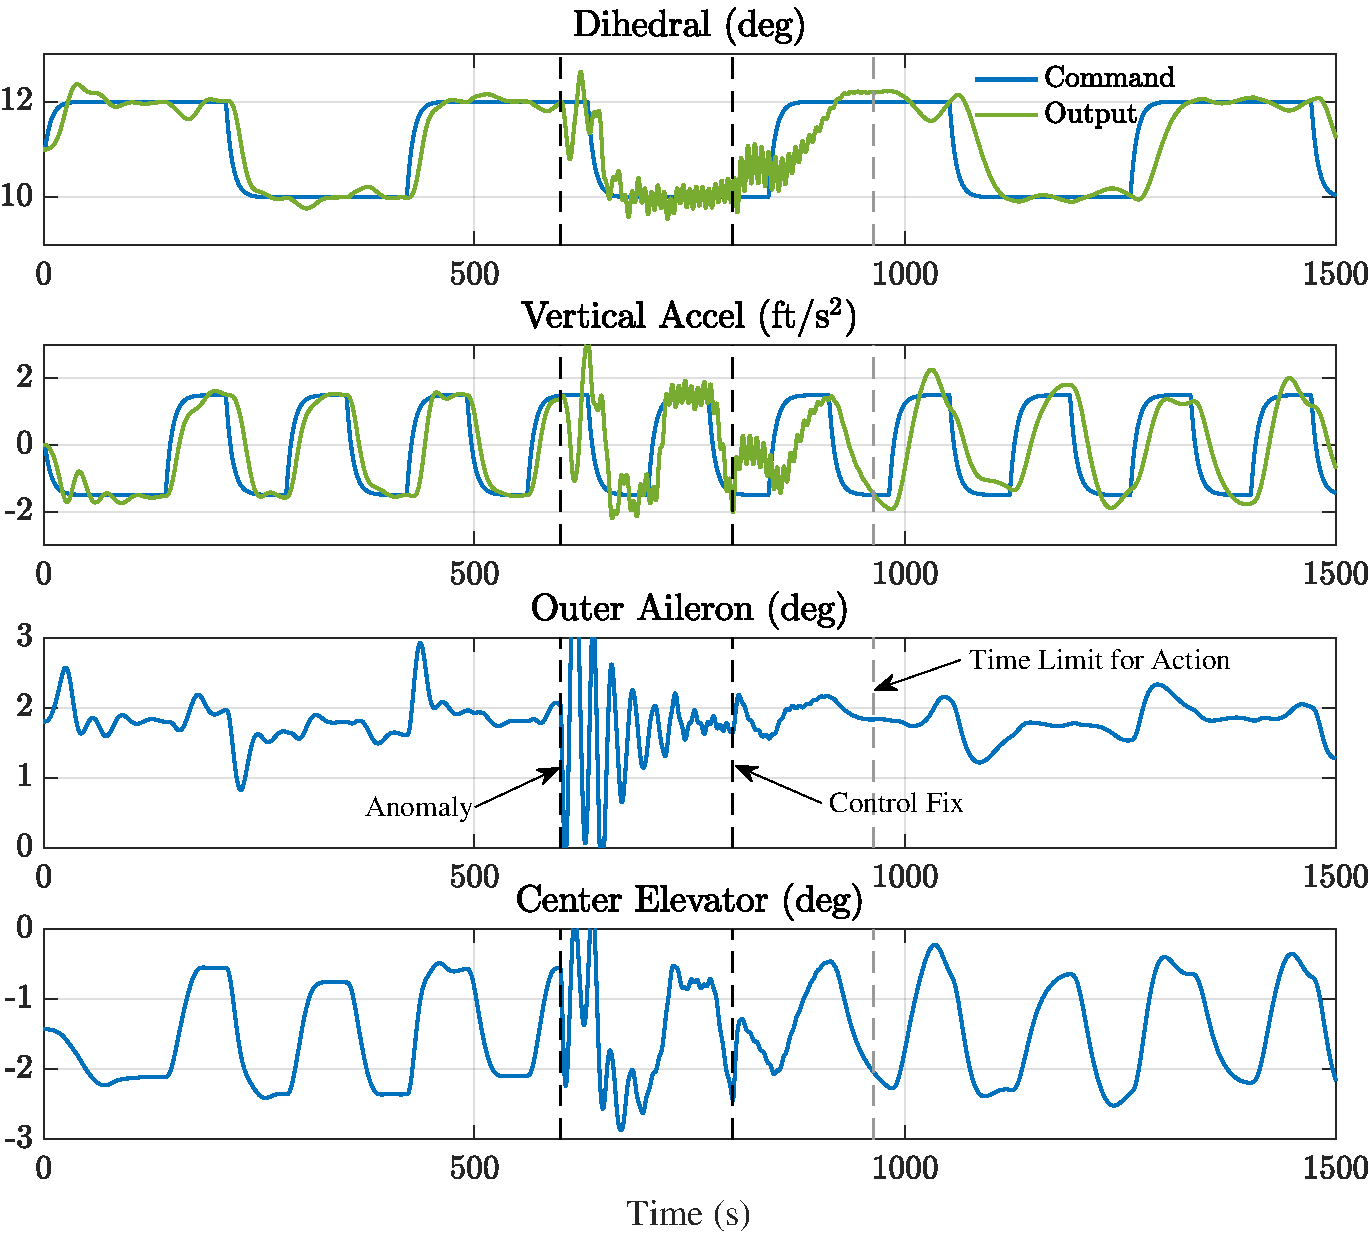
\includegraphics[width=\columnwidth]{ar3.pdf}
	\caption{AR-3 simulation: Shared response to the dynamical anomaly results in recovery of vehicle performance}
	\label{fig:ar3-sim}
\end{figure}

\begin{figure}[htbp]
	\centering
	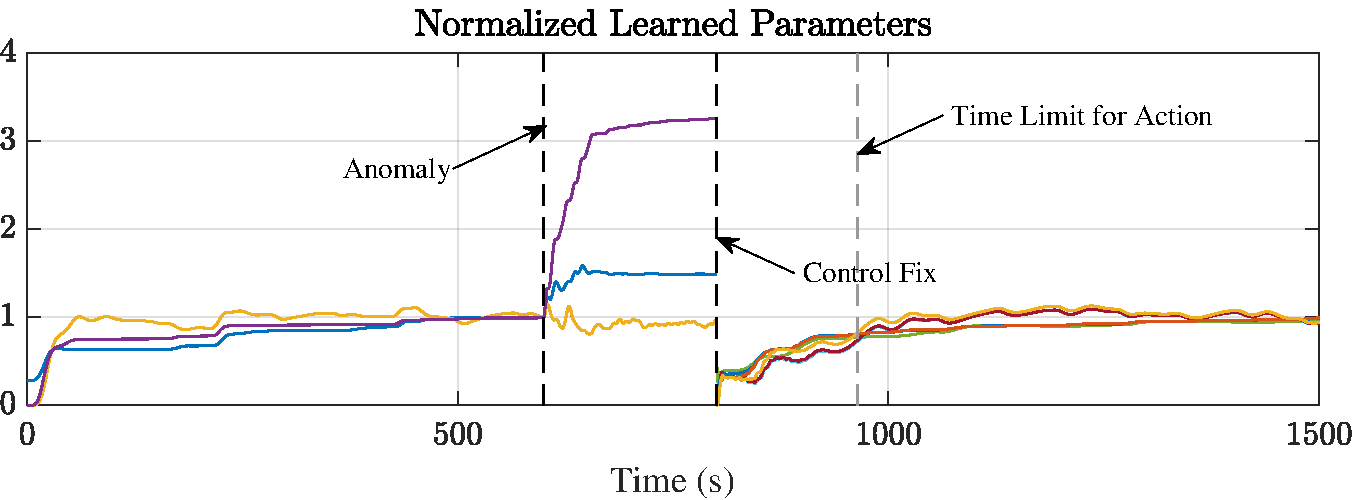
\includegraphics[width=\columnwidth]{ar3-params.pdf}
	\caption{AR-3 simulation: The change in control model at $t_2^* = 800 s$ stops the divergence of adaptive parameters}
	\label{fig:ar3-params}
\end{figure}

\begin{figure}[htbp]
	\centering
	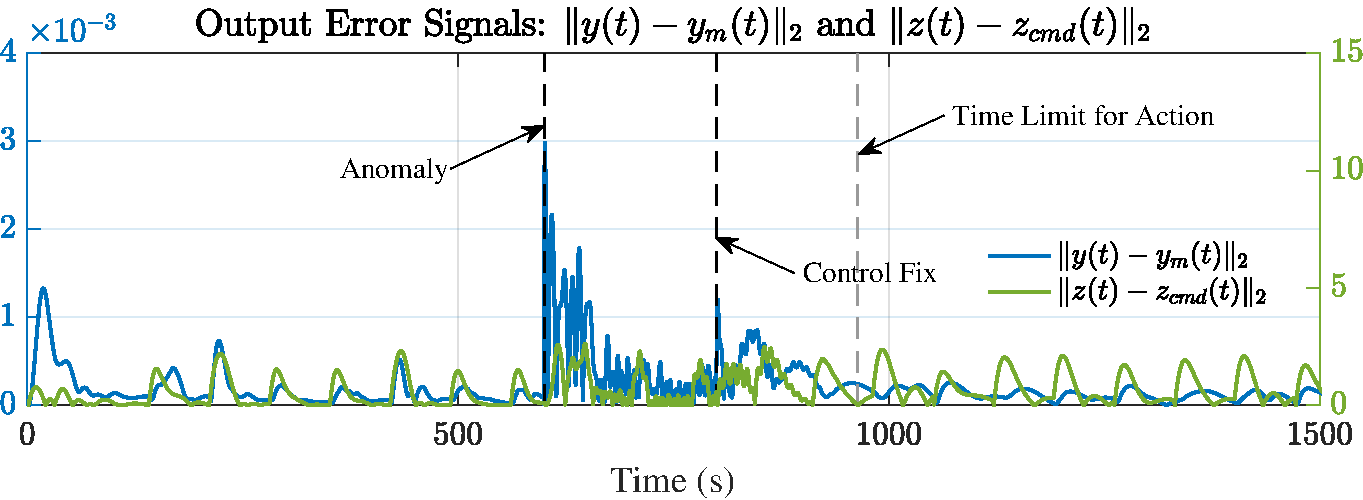
\includegraphics[width=\columnwidth]{ar3-err.pdf}
	\caption{AR-3 simulation: The change in control model at $t_2^* = 800 s$ stops the error growth seen after the anomaly}
	\label{fig:ar3-err}
\end{figure}


\begin{table}[htb]
 \renewcommand{\arraystretch}{1.6}
  \begin{tabular}{>{\raggedright}m{2.2in}|c c c c c}
    \textbf{Simulation} & \textbf{Dynamics Model} & $t_1^*$ & $t_2^*$ & $t_3^*$ & $t_{\textrm{sim}}$ \\
    \hline
    \textbf{Act-AR}: shared control response to actuator lag anomaly & B747 Roll Mode &  30 s & 90 s & N/A & 180 s\\
    \textbf{Del-AR}: shared control response to sensor delay anomaly  & B747 Roll Mode & 30 s & 90 s & N/A & 180 s\\
    \textbf{Del-AR-P}: passive response to sensor delay anomaly  & B747 Roll Mode & 30 s & N/A & 107 s & 180 s\\ \hline
    \textbf{Nom-1}:  nominal VFA command tracking without uncertainty & VFA Pitch Mode & N/A & N/A & N/A & 1500 s\\
    \textbf{Nom-2}: baseline (RSLQR) VFA command tracking with uncertainty & VFA Pitch Mode & N/A & N/A & N/A & 1500 s\\
    \textbf{Nom-3}: adaptive VFA command tracking with uncertainty & VFA Pitch Mode & N/A & N/A & N/A & 1500 s\\ \hline
    \textbf{AR-1}: adaptive VFA command tracking with uncertainty and actuator lag anomaly & VFA Pitch Mode & 600 s & N/A & 960 s & 1500 s\\
    \textbf{AR-1-LQR}: baseline (RSLQR) VFA command tracking with uncertainty and actuator lag anomaly & VFA Pitch Mode & 600 s & N/A & 1240 s & 1500 s\\
    \textbf{AR-3}: shared control response to actuator lag anomaly & VFA Pitch Mode & 600 s & 800 s & N/A & 1500 s\\
  \end{tabular}
  \caption{Summary of the simulations presented in Chapter \ref{ch:numerical}. $t_1^*$ denotes the time of anomaly occurrence, $t_2^*$ denotes the time of the human completing anomaly response tasks, $t_3^*$ denotes the time of plant/controller failure, $t_{\textrm{sim}}$ denotes the simulation length.}
\end{table}

